%%%%%%%% ICML 2026 EXAMPLE LATEX SUBMISSION FILE %%%%%%%%%%%%%%%%%

\documentclass{article}

% Recommended, but optional, packages for figures and better typesetting:
\usepackage{microtype}
\usepackage{graphicx}
\usepackage{subcaption}
\usepackage{booktabs} % for professional tables
\usepackage{diagbox}
% hyperref makes hyperlinks in the resulting PDF.
% If your build breaks (sometimes temporarily if a hyperlink spans a page)
% please comment out the following usepackage line and replace
% \usepackage{icml2026} with \usepackage[nohyperref]{icml2026} above.
\usepackage{hyperref}


% Attempt to make hyperref and algorithmic work together better:
\newcommand{\theHalgorithm}{\arabic{algorithm}}

% Use the following line for the initial blind version submitted for review:
\usepackage{icml2026}

% For preprint, use
% \usepackage[preprint]{icml2026}

% If accepted, instead use the following line for the camera-ready submission:
% \usepackage[accepted]{icml2026}

\usepackage{amsmath}
\usepackage{amssymb}
\usepackage{mathtools}
\usepackage{amsthm}


% if you use cleveref..
\usepackage[capitalize,noabbrev]{cleveref}

%%%%%%%%%%%%%%%%%%%%%%%%%%%%%%%%
% THEOREMS
%%%%%%%%%%%%%%%%%%%%%%%%%%%%%%%%
\theoremstyle{plain}
\newtheorem{theorem}{Theorem}[section]
\newtheorem*{theorem*}{Theorem}
\newtheorem{proposition}[theorem]{Proposition}
\newtheorem{lemma}[theorem]{Lemma}
\newtheorem{corollary}[theorem]{Corollary}
\theoremstyle{definition}
\newtheorem{definition}[theorem]{Definition}
\newtheorem{assumption}[theorem]{Assumption}
\theoremstyle{remark}
\newtheorem{remark}[theorem]{Remark}

\newcommand{\R}{{\mathbb R}}
\newcommand{\Z}{{\mathbb Z}}
\newcommand{\N}{{\mathbb N}}
\newcommand{\E}{{\mathbf E}}
\newcommand{\Var}{{\mathbf{Var}}}
\newcommand{\I}{{\mathbf I}}
\newcommand{\1}{{\mathbf 1}}
\newcommand{\0}{{\mathbf 0}}
%
\newcommand{\A}{{\mathbf A}}
\newcommand{\cA}{{\mathcal A}}
\newcommand{\B}{{\mathcal B}}
\newcommand{\cC}{{\mathcal C}}
\newcommand{\cF}{{\mathcal F}}
\newcommand{\cE}{{\mathcal E}}
\newcommand{\C}{{\mathbf C}}
\newcommand{\F}{{\mathbf F}}
\newcommand{\G}{{\mathcal G}}

\newcommand{\cI}{{\mathcal I}}
% \newcommand{\K}{{\mathcal K}}
\newcommand{\M}{{\mathcal M}}
\newcommand{\cN}{{\mathcal N}}
\newcommand{\cO}{{\mathcal O}}
\newcommand{\cP}{{\mathcal P}}
\newcommand{\bR}{{\mathbf R}}
\newcommand{\Q}{{\mathbf Q}}
\newcommand{\cT}{{\mathcal T}}
\newcommand{\W}{{\mathcal W}}
\newcommand{\X}{{\mathcal X}}
\newcommand{\Y}{{\mathcal Y}}
\newcommand{\cZ}{{\mathcal Z}}
\newcommand{\cR}{{\mathcal R}}

\newcommand{\f}{{\mathbf f}}
\newcommand{\h}{{\mathbf h}}
\newcommand{\z}{{\mathbf z}}
\newcommand{\m}{{\mathbf m}}
\newcommand{\p}{{\mathbf p}}
\newcommand{\q}{{\mathbf q}}
\newcommand{\s}{{\mathbf s}}
\newcommand{\w}{{\mathbf w}}
\newcommand{\x}{{\mathbf x}}
\newcommand{\bu}{{\mathbf u}}
\newcommand{\bv}{{\mathbf v}}

\newcommand{\argmin}{\operatorname{argmin}}

\renewcommand{\>}{{\rightarrow}}

% Todonotes is useful during development; simply uncomment the next line
%    and comment out the line below the next line to turn off comments
%\usepackage[disable,textsize=tiny]{todonotes}
\usepackage[textsize=tiny]{todonotes}

% The \icmltitle you define below is probably too long as a header.
% Therefore, a short form for the running title is supplied here:
\icmltitlerunning{Layers as Lenses: A Narrative of Feature Learning in Deep Networks}


%Newly added packages
% \usepackage[T1]{fontenc}

\begin{document}

\twocolumn[
  \icmltitle{Layers as Lenses: A Narrative of Feature Learning in Deep Networks }

  % It is OKAY to include author information, even for blind submissions: the
  % style file will automatically remove it for you unless you've provided
  % the [accepted] option to the icml2026 package.

  % List of affiliations: The first argument should be a (short) identifier you
  % will use later to specify author affiliations Academic affiliations
  % should list Department, University, City, Region, Country Industry
  % affiliations should list Company, City, Region, Country

  % You can specify symbols, otherwise they are numbered in order. Ideally, you
  % should not use this facility. Affiliations will be numbered in order of
  % appearance and this is the preferred way.
  \icmlsetsymbol{equal}{*}

  \begin{icmlauthorlist}
    \icmlauthor{Firstname1 Lastname1}{equal,yyy}
    \icmlauthor{Firstname2 Lastname2}{equal,yyy,comp}
    \icmlauthor{Firstname3 Lastname3}{comp}
  \end{icmlauthorlist}

  \icmlaffiliation{yyy}{Department of XXX, University of YYY, Location, Country}
  \icmlaffiliation{comp}{Company Name, Location, Country}
  \icmlaffiliation{sch}{School of ZZZ, Institute of WWW, Location, Country}

  \icmlcorrespondingauthor{Firstname1 Lastname1}{first1.last1@xxx.edu}
  \icmlcorrespondingauthor{Firstname2 Lastname2}{first2.last2@www.uk}

  % You may provide any keywords that you find helpful for describing your
  % paper; these are used to populate the "keywords" metadata in the PDF but
  % will not be shown in the document
  \icmlkeywords{Machine Learning, ICML}

  \vskip 0.3in
]
% \maketitle
\printAffiliationsAndNotice{}


\begin{abstract}
% Deep networks with larger number of layers (in the tens typically) significantly outperform shallower counterparts in almost all architecture templates and datasets.  A theoretical and principled reason for their success has eluded the machine learning community over the last decade. Several promising explanations (such as representation power, input space folding, optimization conditioning, and hierarchical feature learning) remain far from being completely proven. We add another potential reason to this list. We hypothesize that, from the perspective of a given layer, other layers in a deep network act as lenses that re-weight the input data. This enables the discovery of features that do not have a global scope and would be missed without the lensing from the other layers. We further describe the feature learning mechanism under gradient descent using a Lure-Trap narrative. It says that network features (when updated by gradient descent) are lured by the decision boundaries of the Bayes optimal classifier close to initialization, based on the strength/scope of decision boundary. Later in training, these decision boundaries act as traps to the model features and do not allow further deviations. This Lure-Trap behavior is made possible mainly because of the hypothesized lensing behavior of the layers. We support our hypothesis/narrative by theoretical arguments and empirical experiments on a recently proposed intrinsically interpretable deep architecture called the deep linearly gated network (DLGN) which takes cues from both deep linear networks and ReLU networks. We also discuss potential reasons for several classic modifications -- pruning, skip-connections, momentum gradient descent -- using our narrative.

% Rewritten using LLMs and tweaked by hand.

Deep neural networks with increasing depth consistently outperform their shallower counterparts across a wide range of architectures and datasets. However, a principled theoretical explanation for this phenomenon remains at a superficial level. While explanations such as representational power, input space folding, optimization conditioning, the neural tangent kernel and hierarchical feature learning have been proposed, they all have glaring deficiencies. We develop a new narrative that postulates the following. From the viewpoint of any given layer, the other layers act as a lens that applies importance weights to the input, facilitating the emergence of features without global scope that would otherwise be overlooked. Gradient methods simply update the parameters of a layer to best fit the data that is importance-weighted by a lens made of other layers. Individual neuron parameters serve a dual role of `separator for data lensed by other layers' and `component of lens for other layers'. This enables a positive feedback loop that forms the core mechanism of feature learning under gradient descent in deep networks. We support our narrative with theoretical analysis and empirical results on the recently proposed Deep Linearly Gated Network (DLGN), an architecture combining elements of deep linear and ReLU networks. We also show how our analysis leads to a natural notion of hierarchical feature discovery in the feature learning regime.
% Our perspective further provides new insights into the effects of architectural modifications such as pruning, skip-connections, and momentum-based optimization.



\end{abstract}


\section{Introduction}
% Writing a narrative in the intro for now will move it to appropriate secions later.

Despite the empirical successes of deep neural networks, prevailing explanations for their learnability remain largely superficial. There exists several popular narratives -- such as ``deeper networks represent more complex functions,'' ``finite-width deep networks approximate infinite-width kernel methods,'' or ``feature kernels evolve to become better during training'' (see, e.g., \cite{Nichani+23, Arora+19, Frei+23}). These accounts overlook why such structures can be reliably learned, fail to address where these explanations break down, and do not explain why empirical phenomena routinely deviate from theoretical predictions. They offer at best, limited insight into some key questions -- 
(1) Why does gradient-based optimization lead to effective solutions?
(2) Why and how do multiple layers enable this behavior?
(3) How is the curse of dimensionality avoided?

A more expressive theory of feature learning is needed to move beyond the current surface-level intuitions and reveal the mechanisms that truly underpin deep learning.

In this paper, we restrict our focus to binary classification problems with feature vector data. Extensions to more complex tasks -- such as generative modelling or structured inputs like images and text -- are beyond the scope of this work. We will also restrict our theoretical arguments to the infinite training data and infinitesimal learning rate setting (corresponding to population gradient flow rather than stochastic gradient descent) for convenience. We strongly believe our arguments can be extended to the SGD setting, but such an extension is beyond the scope of this work. The experiments to support our theoretical arguments are naturally done with finite data and finite learning rate.

\section{Literature Review}

\subsection{An Overview of Current Narratives}

\textbf{Neural Networks and the the Kernel regime:} An important tool for studying the optimization and generalization capabilities of neural networks has been the Neural Tangent Kernel \cite{Jacot+18, Lee+19}. In the infinite-width limit and a certain scaling the network evolution is equivalent to kernel regression given by the NTK. Under this regime, the NTK remains unchanged, making it easier to study the learning dynamics of neural networks \cite{Du+18, Du+19, Arora+18}. The mean-field parameterization \cite{Mei+18, Chizat+18, Bordelon+25} has been a popular alternative to the NTK parameterization since the features evolve under this regime.
% \cite{Geifman+20} showed that the standard Laplace kernel and the NTK are closely related and thus providing a simple tool to study neural networks.

\textbf{Feature learning and gradient descent}: A growing body of work attributes the empirical gap between neural networks trained by gradient descent and kernel methods to the networks’ ability to learn task-relevant features that fixed kernels cannot capture \cite{Zhu+19, Daniely+20, Li+20, Yehudai+19}. Even a small number of gradient steps on the first layer of a two-layer network produces features that improve downstream performance \cite{Daniely+20, Damian+22} . These results are particularly relevant for data that is high dimensional but have a low-dimensional latent structure: in such settings, feature learning effectively reduces the problem to learning the latent subspace. This results in staircase training dynamics formalized in \cite{Abbe+21, Abbe+22b, Abbe+23}. Empirical investigations show that neural networks discover coarse/simple features first and then they progressively capture finer/complex features, consistent with the theoretical staircase picture \cite{Kalimeris+19}. A complementary analytical tool has been to study the evolution of the data-dependent NTK: unlike the fixed NTK of the infinite-width limit, the empirical NTK changes during finite-width training and tends to align with the target, a behavior labeled kernel alignment \cite{Fort+20, Loo+22, Atanasov+22, Wang+23}.

\textbf{The advantage of depth}: Understanding how depth compositionally enhances feature learning remains a central open question. Deeper networks are hypothesized to build a hierarchical representation of features, where the simple features learned by early layers are composed into more abstract concepts by later layers \cite{Allen-Zhu+20}. \cite{Telgarsky+16} show that deep networks cannot be approximated by shallower networks, unless they have an exponentially large number of nodes. \cite{Montufar+14} show that depth enables models to learn a larger number of linear regions thus approximating the target function better than shallower models. \cite{Nichani+23} show that three-layer neural networks have provably richer feature learning capability compared to two-layer networks.

\subsection{Pitfalls of Current Narratives}

The lazy regime of the NTK \cite{Chizat+19} does not explain why neural networks are able to learn complex features from the data. Studies focusing on the feature learning or rich regime -- while providing interesting/useful results -- often consider very simple settings and have restrictive assumptions. For example: only one gradient step, two-layer networks, linear/quadratic activations, layer-wise training schedules, specific initialization scalings, and strong assumptions about the data \cite{Cui+24, Dandi+24, Ba+22, Damian+22, Daniely+20, Abbe+22b}. There is very little understanding on how well these results transfer to deep networks trained end-to-end using gradient descent. The crucial deep learning narrative question -- given below -- remains unanswered to this date. \textit{How do the multiple layers in a deep neural network interact with each other and jointly adapt during training to discover task-relevant features?} A related question of lesser importance is given as follows: \textit{When an architecture and data setting has multiple functionally different global/local minima, how does the initialization relate to the eventual gradient descent solution?} The latter question is  narrower and more technical than the former. Our inability to answer the latter question convincingly for a non-trivial setting makes the former question even harder to grasp.

\section{Decision Tree Data and Deep Linearly Gated Network Architecture}

\subsection{ Motivation for the Data Setting}

A primary goal in selecting a data setting for theoretical study is to ensure genuine non-triviality; the concept class should be complex enough that feature learning via gradient descent on a deep architecture is necessary. While real-world datasets often exhibit this property -- resisting solutions by linear or kernel methods -- their inherent opacity renders precise analysis of model dynamics intractable. By contrast, canonical synthetic benchmarks such as parity functions or linearly separable data or polynomials (see, e.g., \cite{Daniely+20, Frei+23, Soudry+18, Wu+23, Abbe+21} are somewhat simplistic and fail to capture the kind of intricate structure that motivates deep learning theory. Data labeled by an oblique decision tree \cite{Banerjee+25} however, offers synthetic complexity without analytic opacity, furnishing a non-trivial, structured classification task.

An effective data model should permit generalization of its key mechanisms to broader settings, while remaining amenable to precise analysis. Oblique decision trees occupy this middle ground: although real-world datasets are rarely generated by tree processes, many possess rich, multi-scale hierarchical structure that trees can capture or approximate. The essential elements of a decision tree -- its internal node hyperplanes -- can be isolated and interpreted as discontinuities in the label function, regardless of the tree context. As a result, properties established for tree-structured data are more plausibly extended to realistic data regimes than results derived from artificial settings such as parity functions or polynomials. Because oblique trees combine structural expressiveness with analytic tractability, they provide a robust foundation for arguments that aim to reflect the mechanisms enabling deep network success in real data.

\subsection{ Motivation for the Architecture Setting}

To meaningfully advance theory, we require an architecture that is empirically competitive with standard deep networks, such as multilayer ReLU models, on challenging tasks. Classic models favored in theoretical work -- like deep linear networks or single-hidden-layer neural networks -- lack the expressive power and empirical relevance of modern deep architectures. In contrast, the deep linearly gated network (DLGN) achieves close to state-of-the-art performance in feature vector classification tasks \cite{Banerjee+25} and therefore offers a more faithful proxy for understanding deep feature learning in realistic settings.

A suitable architecture should possess a transparent, layer-wise structure whose parameters can be decomposed into interpretable, semi-independent components. While multilayer ReLU networks have a clear notion of depth, the intricate parameter interactions -- especially in intermediate hidden layers -- often render isolated analysis of individual weights or neurons meaningless. This challenge is typically avoided in theoretical studies by restricting consideration to shallow (e.g., single-hidden-layer) networks, sacrificing insights into deep feature learning. The DLGN architecture, by design, enables meaningful dissection of parameter dynamics at the level of individual neurons, while preserving the hierarchical depth necessary for examining deep learning phenomena.

\subsection{The Oblique Decision Tree Data Setting}
\label{sec:ODT_intro}
The instance $\x$ is drawn uniformly from the surface of a sphere of radius one in $\R^d$. The label $y \in\{+1,-1\}$ is given by a complete, orthogonal and balanced oblique decision tree (COB-ODT according to \cite{Banerjee+25}) of depth $D$ which recursively partitions the space at each internal node using orthogonal hyperplanes. Concretely, consider a depth $D-1$ complete binary tree with nodes indexed $0$ to $N = 2^{D}-2$. Each node $i\in\{0,1,\ldots,N\}$ has a left child $2i+1$, and right child $2i+2$. It is also associated with a `decision vector' $\bu_i \in \R^d$. The $N+1$ decision vectors $\bu_0,\ldots,\bu_N$ are unit norm and mutually orthogonal. Traversal starts at the root; at each node $i$, the data point $\x$ proceeds left (right resp.) if the sign of the inner product $\bu_i \cdot \x$ is negative (positive resp.). The label $y^*(\x)$ is  equal to the sign of $-\bu_i\cdot \x$ at the node $i$ reached after $D-1$ decisions. The label nodes are given numbers $N+1$ to $2N+2$ for convenience, even though they do not have an associated decision.  As a convention, we call the nodes at level $D-1$ as leaf nodes, and the nodes at level $D$ as label nodes, e.g. in the depth $D=4$ tree shown in Figure \ref{fig:ODT}, nodes 7 to 14 are leaf nodes, while nodes 15 to 30 are label nodes.

\begin{figure*}
    \centering
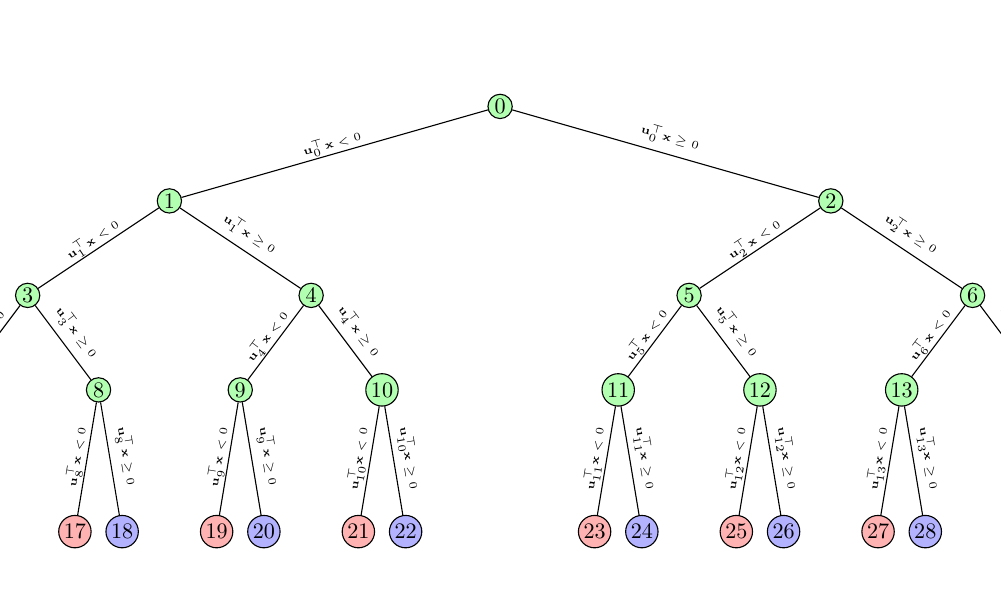
\begin{tikzpicture}[every node/.style={circle,draw,minimum size=10pt,inner sep=1pt, scale=0.8}]

\path[use as bounding box] (-6, -6) rectangle (6, 1);
\begin{scope}[shift={(-0,0)}, scale=0.6]
% Level 0 (root)
\node[fill=green!30] (n0) at (0,0) {0};

% Level 1
\node[fill=green!30] (n1) at (-7,-2) {1};
\node[fill=green!30] (n2) at (7,-2) {2};

% Level 2
\node[fill=green!30] (n3)  at (-10,-4) {3};
\node[fill=green!30] (n4)  at (-4,-4) {4};
\node[fill=green!30] (n5)  at (4,-4) {5};
\node[fill=green!30] (n6)  at (10,-4) {6};

% Level 3
\node[fill=green!30] (n7)  at (-11.5,-6) {7};
\node[fill=green!30] (n8)  at (-8.5,-6) {8};
\node[fill=green!30] (n9)  at (-5.5,-6) {9};
\node[fill=green!30] (n10) at (-2.5,-6) {10};
\node[fill=green!30] (n11) at (2.5,-6) {11};
\node[fill=green!30] (n12) at (5.5,-6) {12};
\node[fill=green!30] (n13) at (8.5,-6) {13};
\node[fill=green!30] (n14) at (11.5,-6) {14};

% Level 4 (leaves)
\node[fill=red!30] (n15)  at (-12,-9) {15};
\node[fill=blue!30] (n16)  at (-11,-9) {16};
\node[fill=red!30] (n17)  at (-9,-9) {17};
\node[fill=blue!30] (n18)  at (-8,-9) {18};
\node[fill=red!30] (n19)  at (-6,-9) {19};
\node[fill=blue!30] (n20)  at (-5,-9) {20};
\node[fill=red!30] (n21)  at (-3,-9) {21};
\node[fill=blue!30] (n22)  at (-2,-9) {22};
\node[fill=red!30] (n23)  at (2,-9) {23};
\node[fill=blue!30] (n24)  at (3,-9) {24};
\node[fill=red!30] (n25)  at (5,-9) {25};
\node[fill=blue!30] (n26)  at (6,-9) {26};
\node[fill=red!30] (n27)  at (8,-9) {27};
\node[fill=blue!30] (n28)  at (9,-9) {28};
\node[fill=red!30] (n29)  at (11,-9) {29};
\node[fill=blue!30] (n30)  at (12,-9) {30};

% Edges
\foreach \i in {0,...,14} {
   \pgfmathtruncatemacro\leftchild{2*\i+1}
   \pgfmathtruncatemacro\rightchild{2*\i+2}
   \draw (n\i) -- (n\leftchild) node[midway, sloped, anchor=south, yshift=-11pt, draw=none] {\tiny{$\bu_{\i}^\top \x <0$}};
   \draw (n\i) -- (n\rightchild) node[midway, sloped, anchor=north, allow upside down, yshift=23pt, draw=none] {\tiny{$\bu_{\i}^\top \x\geq0$}};
}
\end{scope}
\end{tikzpicture}

\caption{The decision tree with depth $D=4$ has its decision nodes shaded green. Label nodes colored red have $y^*=+1$ and label nodes colored blue have $y^*=-1$.}
\label{fig:ODT}
\end{figure*}


Let $\Gamma$ denote the set of paths in the ODT starting at the root $0$ and terminating at a label node. Each element $\gamma \in \Gamma$ is a $(D+1)$-tuple. 
% e.g the depth 4 tree in Figure \ref{fig:ODT} has $16$ elements in $\Gamma=\{(0,1,3,7,15),(0,1,3,7,16), \ldots, (0,2,6,14,30)\}$. 
Let $y^*(\gamma)$ denote the class label corresponding to the path $\gamma$. Every element $\gamma \in \Gamma$ is assoicated with a sign vector $\tau(\gamma) \in \{+1,-1\}^D$ giving the sequence of left/right decisions taken. For example, in the tree shown in Figure \ref{fig:ODT} for $\gamma=(0,1,3,7,15)$, we have $\tau(\gamma)=(-1,-1,-1,-1)$ and $y^*(\gamma) = +1$.

% \begin{equation}
% y^*(\x) = \sum_{\gamma \in \Gamma_+} \prod_{p = 1}^D \1( \tau_p \bu_{\gamma_p} \cdot \x >0)  - \sum_{\gamma \in \Gamma_-} \prod_{p = 1}^D \1( \tau_p \bu_{\gamma_p} \cdot \x >0)
% \label{eqn:ODT_defn}
% \end{equation}

\begin{equation}
\begin{aligned}
y^*(\x) &= \sum_{\gamma \in \Gamma} y^*(\gamma) \prod_{p = 1}^D \1( \tau_p \bu_{\gamma_p} \cdot \x >0) 
\end{aligned}
\label{eqn:ODT_defn}
\end{equation}

where $\tau_p$ is used as a shorthand for the $p$-th element of $\tau(\gamma)$. By construction, for any given $\x$, only one of the paths in $\Gamma$ has a non-zero contribution in the above expression.

% The ODT labeling function is surprisingly difficult for standard learning algorithms. Kernel and linear methods fail completely even for moderate values of $d$ and $D$ (around $100$ and $4$ respectively) \cite{Banerjee+25}, as do conventional greedy decision tree algorithms: the information gain for splitting on the (crucial) root direction $\bu_0$ is zero since the hyperplane $\bu_0 \cdot \x = 0$ bisects the data into perfectly balanced labels in each half. Consequently, greedy methods are myopic and typically miss the global structure. In contrast, deep architectures such as ReLU networks and the Deep Linearly Gated Network (DLGN) \cite{Banerjee+25} can recover the full compositional pattern and achieve high accuracy for even larger values of $d$ and $D$. This makes the ODT setting an ideal case study to analyse the feature learning dynamics in neural networks.

% While the ODT is itself an artificial construction, it offers a rich family of label structures that go well beyond the commonly studied linearly separable data \cite{Soudry+18}, parity functions \cite{Frei+23}, or single-index models \cite{Damian+22}. Its analytic tractability and compositional depth make it a compelling, if challenging, testbed for the theory of feature learning. 


\subsection{The Deep Linearly Gated Network Architecture Setting}
\label{sec:DLGN_intro}
The deep linearly gated network (DLGN) is defined as a sum of products of sigmoidal activation applied to linear functions. Specifically, the model output is
\begin{equation}
    \hat y(\x) = \sum_{\pi \in \Pi} a_\pi \prod_{\ell =1}^L \phi(\w_{\pi,\ell} ^\top \x)
\end{equation}
where $\Pi$ is a discrete index set, $L$ is the number of layers and $\phi:\R\> [0,1]$ is a scaled sigmoid, ($\phi(u)=1/(1+\exp(-\beta u))$). The weight vectors $\w_{\pi,\ell}$ form a total of $|\Pi| L$ vectors in $\R^d$ and constitute the parameters of the model along with $|\Pi|$ scale coefficients $a_\pi$. 

To establish stronger connections with standard deep neural networks, the construction in \citet{Banerjee+25} considers $\Pi = [M]^L$  corresponding to all possible paths across a network with $L$ hidden layers and $M$ neurons per layer. Since the number of such paths grows rapidly with depth and width, the model further restricts parameterization via sharing: for $\pi = (m_1, \ldots, m_L) \in [M]^L$, the weight $\w_{\pi,\ell}$ depends only on the index $m_\ell$ in layer $\ell$, i.e. $\w_{\pi,\ell}  = \w_{m_\ell,\ell}$. \citet{Banerjee+25} also set the scalar coefficients $a_\pi$ as the product of edge weights along the path $\pi$ in an associated deep linear network, i.e. $a_\pi  = \prod_{\ell=2}^L a_{\ell,m_{\ell-1},m_{\ell}}$.  

The total number of parameters involved in the above setting is $ML$ for the gating neurons $\w_{m,\ell}$, and $(L-1)M^2$ for the path coefficient parameters $a_{\ell,m_1,m_2}$. This setting also enables efficient model output computation (complexity $O(M^2 L)$) without explicitly summing over $M^L$ paths.


Despite its structural simplicity compared to standard ReLU networks, the DLGN has proven to be a surprisingly powerful learning architecture \cite{Banerjee+25}. It maintains a transparent correspondence between parameters and their effect on the output -- each $\w_{i,\ell}$ represents a component whose influence on $\hat y$ can be traced directly. 

% It mirrors the notion of layers and neurons from standard ReLU networks, while allowing detailed theoretical analysis.

% The rest of the paper analyzes the dynamics of parameters of the DLGN model under gradient descent over the log-loss with ODT labeled data. For the sake of simplicity, we assume infinite data and infinitesimal learning rate, i.e. population gradient flow. 

% But all our simulations are with training size ten to hundred times the number of parameters as the ODT model, i.e. $Nd = 2^Ld$, and learning rate set to the largest value for which the training loss curve remains smooth.

% We find it useful to split our analysis of the DLGN learning dynamics into a `Lure' phase and 'Trap' phase. The lure phase is applicable early in training, when the gating features/half-spaces have not discovered anything substantial. More concretely, when the effective weights $V^\ell$


\section{Learning Dynamics of Single Path DLGN}
\label{sec:single-path-DLGN}
Consider the single path DLGN, with $M=1$. While this is not a useful architecture by itself, it still exhibits interesting behavior that is illustrative of the message we intend to convey for deep architectures in general. Precisely, we consider the model
\[
\hat y(\x; a, W) = a \prod_{\ell =1}^L \phi(\w_\ell ^\top \x)
\]
with parameters $a \in \R, \w_1 , \ldots, \w_L \in \R^d$. We concatenate the $L$ gating vectors $\w_1, \ldots, \w_L$ together as a single vector $W \in \R^{Ld}$ for convenience. Let $P_\ell:\R^d \>\R^{Ld}$ be such that $P_\ell(\bu)$ sets the $\ell$-th $d$-dimensional block of the output equal to $\bu$ and zero elsewhere. %For example, $W = P_1(\w_1) + \ldots + P_L(\w_L)$.

This model is not powerful enough to fit the ODT labeled data. But the form of the model suggests that it might `capture' one of the paths of the ODT labeling function. The analysis for establishing this is worthy of a deep dive.

\subsection{Lens and Blinders}
The main tool that enables our analysis, is the loss gradient with respect to one of the weight vectors (say) $\w_k$. Consider the loss gradient for a single data point $(\x,y^*)$. 

\begin{align}
\mathcal{L}(\hat y(\x)) 
&= \log(1+\exp(-y^* \hat y(\x))) \nonumber \\
% \frac{\partial L(y^*,\hat y(\x))}{ \partial \w_k}  
% &=  \sigma (-y^* \hat y(\x)) (-y^*) \frac{\partial \hat y(\x)}{ \partial \w_k}\nonumber\\
-\nabla_{\w_k} \mathcal{L} &=  \E [ \underbrace{\sigma (-y^* \hat y(\x))}_{\text{Residue}} 
 \underbrace{ \Lambda_k(\x) }_{\text{Lens}}  \underbrace{\phi'(\w_k ^\top \x)}_{\text{Blinder}} y^* a\x ]\label{eqn:ResidueLensBlinder}
\end{align}
where $\Lambda_k(\x)=\prod_{\kappa \neq k} \phi(\w_\kappa ^\top \x)$. The negative loss gradient w.r.t. $\w_k$ is a positive scalar multiple of $y^*a\x$ . 
% This scalar is broken into a product of three terms in Equation \eqref{eqn:ResidueLensBlinder}, which we call the residue, lens and blinder. 

The gradient descent step for $\w_k$ can now be viewed as a Perceptron-like update over the entire training dataset $S$, with importance weights to a sample $\x,y$ given by the product of the residue, lens and blinder terms. While $\w_k$ is updated to fit the data that is importance weighted based on its lens, it also acts as a component of the lens for other neurons. 
% This is the key dynamic that allows for interactions between the different layers. 
% The value of this interaction is as follows. 
% Important features without a global scope (like the root node of the ODT $\bu_0$) would not contribute anything to the gradient in the absence of a lens term. 
With the right lens, the gradient will have a strong component along feature directions that do not have a global scope (like the ODT root node $\bu_0$). This dual role of  `component of  lens for other layers' and  `linear separator for data lensed by other layers' served by the vectors $\w_k$ forms a positive feedback loop.

\subsection{Second Order Analysis}
\label{sec:second_order_analysis}
% A main goal in the paper is to analyze the feature learning dynamics of gradient descent in deep networks. A standard interpretation of `feature' in deep networks would be the Neural Tangent Kernel features, which are simply a property of parameter gradients of the model output \cite{Jacot+18}. Any analysis of `feature learning' would thus have to study how the NTK features change during training,  which essentially corresponds to performing (at least) a second order analysis. 

A natural choice for analyzing `feature learning' is to study how the NTK features change during training, which corresponds to performing a second order analysis.  We  specialize the analysis of the gradient to the ODT labelled data, where $y^*$ is given by Equation \ref{eqn:ODT_defn} and show how the positive feedback between the two roles of a neuron $\w_k$ enables better learning of the ODT features by the model. 
% We fix the DLGN scaling parameter $a$ to be a constant in our result below, and only view the loss $\mathcal{L}$ as a function of $W$.


\begin{theorem}[Hierarchy seeking lens]
\label{thm:second_order_lens}
Let $\h, \z  \in \R^d$. Let $0<a<1, k\neq \ell$. Let $\w_\lambda^\top \h = \w_\lambda^\top \z = 0$ for all $\lambda \in [L]$. The change in gradient of $\mathcal{L}$ w.r.t. $\w_k$ along $\z$,   as $\w_\ell$, moves along $\h$ satisfies
% \[
%  -\h^\top  \big[\nabla^2_{\ell,k} L(W) \big] \z =  \lim_{\epsilon \> 0} \frac{1}{\epsilon} \bigg[ -\nabla_{\w_k} L(W + \epsilon P_\ell(\h)) \cdot \z  + \nabla_{\w_k} L(W) \cdot \z \bigg] > 0
% \]

\begin{align*}
\lim_{\epsilon \to 0} \frac{1}{\epsilon} \bigg[ 
 -\nabla_{\w_k} \mathcal{L}(W + \epsilon P_\ell(\h))  
 + \nabla_{\w_k} \mathcal{L}(W)  \bigg]\cdot \z > 0
\end{align*}

where $\z= s \bu_i, \h = \bu_j$,  $j\in\{N/2,\ldots,N\}$ is a leaf node of the ODT, and $i$ is any ancestor of $j$. The scalar $s=+1$ if $j$ is in the left sub-tree of $i$ and $-1$ otherwise. The above inequality also holds when $\h$ and $\z$ are swapped.
\end{theorem}

% The structure of gradient descent ensures that $\w_k$ moves along $-\nabla_{\w_k} L(W)$.  Thus,  $\big[ -\nabla_{\w_k} L(W + \epsilon P_\ell(\h)) \cdot \z  + \nabla_{\w_k} L(W) \cdot \z \big]$ captures the extra push that $\w_k$ receives to move along $\z$ when $\w_\ell$ moves along $\h$. 

An example implication  of Theorem \ref{thm:second_order_lens} follows.  If $\w_\ell$ moves along $-\bu_j$ for some leaf node $j$ on the left side of the root node $0$, then $\w_k$ is pushed along $-\bu_0$. This tendency of gradient descent to push a neuron based on the movement of another neuron is fundamental to the feature learning dynamics of the DLGN -- and plausibly to all multi-layer non-linear architectures. This enables the model to handle the curse of dimensionality -- i.e. even in a worst case initialization where all the neurons $\w_k$ are orthogonal to all the ODT directions $\bu_i$, the neurons evolving under gradient descent have a chance of capturing the ODT features $\bu_i$ corresponding to non-leaf nodes $i$. The gradient at initialization has little to no component along these $\bu_i$ at initialization. Without the kind of second order mechanism described by Theorem \ref{thm:second_order_lens} these decision vectors which are crucial for good generalization performance will not be captured. 

%This is much less of a serious problem at lower values of $d$ --  the initialization is quite likely to have some component along $\bu_i$.

Under a symmetric initialization (like $W=0, a>0$), gradient descent will hit a saddle point $W^*$,  corresponding to each of the $L$ neurons taking the same vector $\w^* = c \sum_j -\bu_j$,  where $j$ ranges over leaf node indices $N/2$ to $N$.  However,  the second order dynamics in Theorem \ref{thm:second_order_lens} ensure that with a little asymmetry a positive feedback loop kicks in. A detailed example is discussed in Section \ref{sec:single_trajectory}

%Theorem \ref{thm:second_order_lens} captures the important early phase of training, when the initial weights $\w_\ell$ have no correlation with the relevant data features $\bu_j$. It aligns with goals of the learner and is a desirable property of deep networks and captures a key reason for its success. However, 
Second order dynamics of gradient descent in this problem also has a potentially undesirable behavior.


\begin{theorem}[Self-opposing Lens]
\label{thm:second_order_backlash}
Let $\h$ be a vector in $\R^d$ that is orthogonal to the ODT decision vectors $\bu_i$ for all $i \in \{0,1,\ldots,n\}$. 
% Let the lens for layer $k$ be at most mildly positively correlated with the label $y$, i.e. $\E[\Lambda_k(\x) y ] < \frac{1}{N}\E[\Lambda_k(\x)]$. 
Let $\w_\lambda \cdot \h = 0$ for all $\lambda \in\{1,\ldots,L\}$. Let $\w_\lambda \cdot \bu_j = 0$ for all $\lambda \in\{1,\ldots,L\}$ and $j \in \{N/2,\ldots, N\}$. The change in gradient of $\mathcal{L}$ w.r.t. $\w_k$ along $\h$  as $\w_\ell$ (for some $\ell \neq k$) moves along $-\h$ satisfies the following relation.

% \[
%  \h^\top  \big[\nabla^2_{\ell,k} L(W) \big] \h =  \lim_{\epsilon \> 0} \frac{1}{\epsilon} \bigg[ -\nabla_{\w_k} L(W + \epsilon P_\ell(\h)) \cdot (-\h)  + \nabla_{\w_k} L(W) \cdot (-\h) \bigg] > 0
% \]

\begin{align*}
\lim_{\epsilon \to 0} \frac{1}{\epsilon} \bigg[ 
 -\nabla_{\w_k} \mathcal{L}(W + \epsilon P_\ell(\h))  
 + \nabla_{\w_k} \mathcal{L}(W)  \bigg]\cdot (-\h) > 0
\end{align*}
\end{theorem}

% Refer Appendix \ref{app:second_order_backlash} for detailed proof. 
In words,  Theorem \ref{thm:second_order_backlash} says that if some neuron $\w_\ell$ moves along some $\h$, the tendency of other neurons $\w_k$ to move along $-\h$ increases. For example, if for some reason (due to say finite data imbalances or some initial perturbation), some neuron $\w_\ell$ is moved along a direction $\h$ that is spurious from a generalisation perspective (e.g. $\h \cdot \bu_i =0$ for all $i$) then other layers tend to move along $-\h$ and the component of the gating vectors along $\h$ and $-\h$ keep increasing. Informally,  each neuron tries to correct for mistakes in some other layers' neuron, and becomes part of the mistake that other neurons try to correct.  The problematic nature of this behaviour becomes apparent only in the multi-path DLGN with deeper ODT label functions.  We will discuss this further in Section \ref{sec:gating_regularization}.
 
Theorems \ref{thm:second_order_lens} and \ref{thm:second_order_backlash}, is approximately applicable at most initialization for the large $d$ setting, i.e. $d >> 2^D$. The initial weight vectors then are quite likely to be close to orthogonal to all the ODT vectors. It is also applicable at the zero initialization $W=0$. The second order quantity in these theorems is a continuous function of the parameters $W$, and hence can clearly be extended to hold beyond strict orthogonality. Analysis of the exact amount of orthogonality relaxation under which the Theorems still hold is beyond the scope of this paper. The insights from Theorems \ref{thm:second_order_lens} and \ref{thm:second_order_backlash} are valid well beyond their restrictive orthogonality assumptions -- the second order dynamics are merely responsible for pushing the parameter into an appropriate basin in the loss landscape, and hence do not need to hold strongly throughout training. We support this argument in Sections \ref{sec:single_trajectory} and \ref{sec:trajectory_prediction} where we use the hints from the hierarchy-seeking lens and self-opposing lens at initialization, to successfully predict the result of gradient descent training.
%For example, if $|\w_\kappa .\bu_0|$ is already large for some $\kappa$, then there is no need for some other layer $\w_k$ to move along $\bu_0$.

\subsection{Trajectory Analysis for a Chosen Initialization}
\label{sec:single_trajectory}

\begin{figure*}
\includegraphics[width=1.05\textwidth]{figs/Single_path_DLGN/parameter_trajectory_0178_400epochs.pdf}
\includegraphics[width=1.05\textwidth]{figs/Single_path_DLGN/gradient_trajectory_0178_400epochs.pdf}
\caption{The parameter and gradient trajectories as a function of training time.}
\label{fig:single_trajectory_0178} 
\end{figure*} 

In this Section (and the next) we consider the ODT labelling function with depth $D=4$ in Figure \ref{fig:ODT}, and a single path DLGN with $L=D=4$ layers.  We focus on the solutions to weight vectors $\w_\ell$ and freeze the scalar coefficient $a=1$. We analyse in detail how Theorem \ref{thm:second_order_lens} and \ref{thm:second_order_backlash} determine the parameter trajectory under gradient flow from a given initialization. All of this analysis can be extended to deeper trees and DLGNs as well. 

Firstly note that $a>0$ means the model can achieve non-trivial log loss (loss values less than $\log(2)$) only on positive labelled points, i.e. data reaching label nodes $15,17,\ldots,29$. All these label nodes lie on the left side of their parents. Thus, when a DLGN is initialized with $W=0$ and $a>0$, gradient descent pushes all $\w_k$ along $\sum_j -\bu_j$, where $j$ takes on leaf node indices $N/2$ to $N$. This happens till the parameter $W$ reaches the saddle point $W^*$ and stays there. The gradient has no component along any other direction due to symmetry.    

But, the properties of the loss landscape $\mathcal{L}(W)$ (mainly relating to Theorem \ref{thm:second_order_lens}) cause interesting things to happen even under a slight perturbation in an appropriate direction. Let the parameter $W$ be initialized to a perturbation of the fully symmetric zero initialization, such that
$\w_1 = \0$, 
$\w_2 =  - \epsilon \bv $,
$\w_3 =  - \epsilon \bv -\epsilon \bu_7$,
$\w_4 =  - \epsilon \bv -\epsilon \bu_8$. 
for some small $\epsilon>0$ and $\bv = \bu_7+\bu_8+\bu_9+\bu_{10}$. The parameter and gradient trajectories with this initialization is given in Figure \ref{fig:single_trajectory_0178}. This infinitesimal push from $\0$ starts a feedback loop between the neurons in different layers. The perturbation directions above were carefully chosen based on Theorem \ref{thm:second_order_lens}. From the perspective of $\w_1$, all the other layers have moved along $-\bu_7, -\bu_8, -\bu_9$ and $-\bu_{10}$. Thus Theorem \ref{thm:second_order_lens} says that $\w_1$ experiences an increased push towards $-\bu_0$. Now consider the version of Theorem \ref{thm:second_order_lens} with $\h$ and $\z$ swapped.  This movement of $\w_1$ towards $-\bu_0$ pushes all the other layers further along the leaf node ODT directions and hence completes a feedback loop. Meanwhile, the minor extra movement of $\w_3$ and $\w_4$ along $-\bu_7$ and $-\bu_8$ at initialization cause $\w_2$ to move along $-\bu_1$ from Theorem \ref{thm:second_order_lens}. This tendency of $\w_2$ to move along $-\bu_1$ is weak at initialization, and becomes stronger only after $\w_1$ has moved sufficiently along $-\bu_0$. The neurons $\w_k$ have a natural self-inhibitory tendency as indicated by Theorem \ref{thm:second_order_backlash} which causes $\w_1$ moving along $-\bu_0$ to dissuade other neurons from doing the same -- in fact the other layers move slightly along $+\bu_0$ around the same time as $\w_1$ experiences its largest push towards $-\bu_0$. Even though all the neurons have an increased tendency to move along $-\bu_0$ at initialization, this effect is strongest for $\w_1$. 

% Also, note that in the early stages, the second order effects from \ref{thm:second_order_lens} are yet to fully kick in, and the parameter movements are primarily determined from the first order dynamics that take the model from $W=0$ to the saddle point $W=W^*$. As long as the perturbation remains directionally intact at the end of this beginning phase, the second order dynamics from Theorems \ref{thm:second_order_lens} and \ref{thm:second_order_backlash} become active long enough to push the parameter into the corresponding solution basin in the optimization landscape.

Now we can read the parameter trajectories under gradient descent shown in Figure \ref{fig:single_trajectory_0178}. The initialization scale $\epsilon$ is too small to be seen on the plot. The first 10 epochs correspond to the parameter movement from the initialization close to zero to the saddle point at $W^*$. The effect of second order dynamics from Theorem \ref{thm:second_order_lens} begin to be visible only from this point. From around epoch 10 to 50  the gradient component of $\w_1$ along $-\bu_0$ keeps increasing. From around epoch 50 to 90, the gradient component of $\w_2$ along $-\bu_1$ keeps increasing. The neurons $\w_3$ and $\w_4$ which were closer to $-\bu_7$ and $-\bu_8$ at initialization grow along $-\bu_7$ and $-\bu_8$ respectively. The final gradient descent convergent solution is closely approximated (up to a scaling factor) by $\w_1 = -\bu_0, ~ \w_2 = -\bu_1,~ \w_3 = -\bu_7+0.3\bu_3$ and $ \w_4 = -\bu_8-0.3 \bu_3$, as can be seen in Figure \ref{fig:full_trajectory} in the Appendix. This corresponds  to a superposition of two adjacent ODT paths to a positively labelled node -- corresponding to $-\bu_0, -\bu_1, -\bu_7, -\bu_3$ and $-\bu_0, -\bu_1, +\bu_3, -\bu_8$. There are 4 such solutions, corresponding to the 2 leaf nodes being $7,8$ or $9,10$ or $11,12$ or $13,14$. Each of these 4 solutions can appear in $4!=24$ configurations due to permutation invariance of the layers in the DLGN model. Thus making for a total of 96 solutions in the parameter space (or $2^{D-2}D!$ in general with $D=L$). One can easily design minor perturbations of $W=0$ that reach any of these solutions under gradient descent. 

We will use a $D$-tuple to compactly represent the $2^{D-2}D!$ solutions, based on the argmax of absolute value of the projections of the neurons along the ODT directions. i.e for a solution $\tilde W \in \R^{D \times d}$ its representation $\upsilon(\tilde W) \in \{0,1,\ldots,2^{D}-2\}^D$ is 
\[
\upsilon_\ell(\tilde W) = \text{argmax}_{i \in \{0,\ldots,2^D-2\}} |\w_\ell \cdot \bu_i|.
\]
For example, if $\tilde W$ is the convergent solution to the trajectory illustrated in Figure \ref{fig:single_trajectory_0178}, then $\upsilon(\tilde W) = [0,1,7,8]$.
 

%The parameter trajectory is explained and the initial perturbations are designed mainly through the insight from Theorems \ref{thm:second_order_lens} and \ref{thm:second_order_backlash}. Both these theorems are not strictly applicable at any point in the solution trajectory beyond the zero initialization due to the orthogonality requirements. However, they likely remain valid for much longer enabling a coherent narrative explaining the entire parameter trajectory. 




\subsection{Solution Prediction from Random Initialization}
\label{sec:trajectory_prediction}

% Again, let us consider the ODT problem with depth $D=4$ in Figure \ref{fig:ODT}, and a single path DLGN with $L=4$ layers.  We focus on the solutions to weight vectors $\w_\ell$ and freeze the scalar coefficient $a=1$.

Constructing bespoke initializations close to zero that make parameter trajectory go to any of the solutions demonstrates a level of control and understanding over the gradient descent dynamics. However, in typical random initializations, the perturbations from $\0$ are not going to perfectly match one of these canonical perturbations. A typical scenario might have initialization supporting multiple solutions simultaneously. Assuming that gradient descent takes such a  random initialization to one of the $96$ solutions, which is it?

%Firstly, we should note that a significant fraction (about half, based on our experiments) of the initializations remain stuck in $W^*$ or some other saddle point. We will ignore such initializations in our analysis.\footnote{In all such runs the training loss saturates at a level between $\log(2)$ and $\frac{15}{16}\log(2)$}. Even for trajectories that reach one of the 96 solutions, we do not yet have a full comprehensive theory of why gradient descent takes $W$ to that solution from the corresponding initialization. 

We do not have a full answer for this question. However, we can design heuristics that use Theorem \ref{thm:second_order_lens} and \ref{thm:second_order_backlash} to `measure' the support the initial parameter $W(0)$ gives to each of the $96$ solutions. The details of this heuristic score construction are  somewhat intricate and given in Appendix \ref{sec:appendix_heuristic_score}. Briefly, it is the sum of three terms -- a term measuring the proximity of the init to a solution, a term measuring the hierarchy seeking lens' support weighted by a scalar $c_{\text{HS}}\geq 0$,  and a term measuring the self-opposing lens' support weighted by a scalar $c_{\text{SO}}\geq 0$. 


We run gradient descent for the single path DLGN with $2000$ different initializations, each with 5 different datasets sampled from the same distribution. This is done to ensure that the gradient descent convergent solution is purely a property of the initialization, and not any finite data effects. $368$ of these initializations passed the test -- i.e. the gradient descent convergent solution for these initializations did not change with data. The parameters $c_{\text{HS}}, c_{\text{SO}}$ of the score function were searched from $0.0$ to $0.9$ in increments of $0.1$ for a total of 100 possible configurations. The best performing coefficients (which happened to be $c_\text{SO}=0.7, c_\text{HS}=0.4$) gave the correct solution for $179$ out of these $368$ initializations (corresponding to an accuracy of $49\%$ for a $96$-class classification problem). 

A baseline predictor that just predicts the solution nearest to initialization (corresponding to $c_\text{SO}=0, c_\text{HS}=0$) achieves a prediction accuracy of $13\%$. In particular, both the hierarchy-seeking and self-opposition components are crucial to the score -- the best accuracy when setting $c_\text{HS} = 0$ (resp. $c_\text{SO} = 0$) is $28\%$ (resp. $36\%$). This makes our notion of `layers as lenses' a viable explanation of the learning dynamics of the DLGN. 


\section{The Multi-Path DLGN}
\label{sec:multi-path-DLGN}

\begin{figure*}
\begin{center}
\includegraphics[width=0.33 \textwidth]{figs/Multi_path_DLGN/Regularization_0_phase1/Epoch_0.pdf}
\includegraphics[width=0.33 \textwidth]{figs/Multi_path_DLGN/Regularization_0_phase1/Epoch_1000.pdf}
\includegraphics[width=0.33 \textwidth]{figs/Multi_path_DLGN/Regularization_2e-4_phase1/Epoch_1000.pdf}    
\end{center}
\caption{Gating norms vs cosine sim. to ODT vectors at (a) the beginning of training (b,c) end of training without and with L2 penalty.}
\label{fig:norms_cosine_scatter_no_reg_final}
\end{figure*}

\begin{figure*}
\begin{center}
\includegraphics[width=0.33\textwidth]{figs/Multi_path_DLGN/Regularization_2e-4_phase1/Epoch_1.pdf}
\includegraphics[width=0.33\textwidth]{figs/Multi_path_DLGN/Regularization_2e-4_phase1/Epoch_3.pdf}
\includegraphics[width=0.33\textwidth]{figs/Multi_path_DLGN/Regularization_2e-4_phase1/Epoch_5.pdf}
\end{center}
\caption{Gating norms and cosine similarity to ODT  vectors during training (with the L2 penalty).}
\label{fig:hieararchical_feat}
\end{figure*} 

\begin{figure*}
\begin{center}
\includegraphics[width=0.33 \textwidth]{figs/ReLU_3layer/Epoch0_Update0.pdf}
\includegraphics[width=0.33 \textwidth]{figs/ReLU_3layer/Epoch0_Update100.pdf}
\includegraphics[width=0.33 \textwidth]{figs/ReLU_3layer/Epoch0_Update999.pdf}    

\includegraphics[width=0.33 \textwidth]{figs/ReLU_3layer/3.pdf}    
\includegraphics[width=0.33 \textwidth]{figs/ReLU_3layer/40.pdf}    
\includegraphics[width=0.33 \textwidth]{figs/ReLU_3layer/400.pdf}    
\end{center}
\caption{Gating norms vs cosine similarity of first layer ReLU neurons to ODT vectors at different points in training.}
\label{fig:norms_cosine_scatter_ReLU}
\end{figure*}


In this section we consider the more practical multi-path DLGN with $M>1$. Setting $M=1$ upper bounds the representative power of the DLGN -- it can at best capture ODT data entering one leaf node, which corresponds to low loss on $\frac{1}{2^D}$ fraction of the data, and close to random performance on the rest of the data. Larger width DLGN models do not suffer from this problem.  For example, in this section we will consider a setting of $100$ dimension, depth $5$ ODT labelled data, and a $5$-layer DLGN model having $16$ nodes per layer, i.e $d=100, D=5, L=5, M=16$. It is possible to achieve low losses and error rates on the entire data using such models. We note that no linear/kernel/tree based method perform satisfactorily (error rates remain $> 30\%$) for this data. Thus this data is an example that shows successful feature learning by deep models. See Appendix \ref{app:performance} for a comparison of DLGN with other models.

\subsection{Effect of Gating Regularization}
\label{sec:gating_regularization}

Let the DLGN model be trained under a standard set-up where the log loss (over both the scaling parameters $a$ and gating parameters $\w$) is minimized using a gradient descent method. This gives reasonable performance -- the train loss goes down from $\log(2)=0.69$ at initialization to around $0.05$. The test error rate goes from $50\%$ at initialization to about $10\%$. This would be the end point for a standard architecture (like the ReLU network), or some other dataset (like CIFAR10) as no further debugging/performance analysis is possible -- only mindless hyperparameter tuning till we get better performance.  


However, we are training a DLGN model on the ODT dataset, and hence we know exactly what the desirable learning behaviour is -- as training progresses the gating vectors $\w_{m,\ell}$ should increase in norm along one of the ODT decision vectors $\bu_j$. It is clear that any component of $\w_{m,\ell}$ along a direction orthogonal to all $\bu_i$ can be of no help in learning the target function. Figure \ref{fig:norms_cosine_scatter_no_reg_final}(b) gives a scatter plot showing how the $16*5=80$ neurons are at the end of training. The x-axis corresponds to the norm of the gating vector, and the y-axis corresponds to the max cosine similarity  with any of the ODT vectors. A corresponding figure for the same before training begins is given in Figure \ref{fig:norms_cosine_scatter_no_reg_final}(a). We can see that a significant fraction of the neurons have high norms, but do not correspond to any of the ODT vectors. This is clearly undesirable behaviour. 



We conjecture that, a major component of this undesirable behaviour is from Theorem \ref{thm:second_order_backlash}, where one neuron moving along a spurious direction makes other neurons move in spurious directions too. If this is indeed the reason for the undesirable behaviour, a potential fix might be to add an L2 penalty term for the gating norm to the objective, instead of pure cross entropy loss. Note that the L2 penalty term is not intended to be a regulariser for improving test performance, but rather it is designed to remove undesirable structures in the training loss optimisation landscape. This simple change to the objective causes a significant change in the optimization behavior. The resulting scatter plot showing gating vector norms and cosine similarity to the ODT decision vectors at the end of training with a L2 penalty is given in Figure \ref{fig:norms_cosine_scatter_no_reg_final}(c). Almost all large norm gating vectors are aligned with one of the ODT decision vectors. 

%\begin{figure}
%\includegraphics[width=0.48 \textwidth]{Figs/Multi_path_DLGN/Regularization_2e-4_phase1/Epoch_0.pdf}
%\includegraphics[width=0.48 \textwidth]{Figs/Multi_path_DLGN/Regularization_2e-4_phase1/Epoch_1000.pdf}
%\caption{Gating vector norms and cosine similarity to ODT decision vectors at the beginning and end of standard training.}
%\label{fig:norms_cosine_scatter_with_reg_final}
%\end{figure}

However, this L2 penalty restricts the gating vectors from also moving along the ODT decision vectors, and thus converges to a worse training loss of $0.2$ and a test error of $15\%$. We propose a natural modification to keep the benefits of regularization, while also letting the gating vectors grow in norm. We simply restart training with the L2 penalty convergent solution as the initialization, and remove the L2 penalty in this second phase of training. Additionally, during the initialisation we also forcibly set gating vectors below a threshold norm to $0$ and keep it fixed throughout the second phase of training. This is motivated from Figure \ref{fig:norms_cosine_scatter_no_reg_final}(c) which suggests we can retain most of the `useful' gating vector simply by thresholding based on their norms. 
This modification is successful and reduces the test error further to around $5\%$. Note that this is a legitimate training strategy, as we never explicitly use the ODT vectors in the training procedure and only use it in the scatter plots to illustrate the problem and motivate a modification to standard gradient descent.




\subsection{Hierarchical Feature Emergence}
\label{sec:hierarchical_feature_emergence}



Looking into the learning dynamics of the multi-path DLGN with a L2 penalty on the gating vectors, we find interesting details that support our narrative of feature learning established in Section \ref{sec:single_trajectory}. Figure \ref{fig:single_trajectory_0178} suggests that the initial movement of the gating vectors is along the leaf node decision vectors until it reaches a saddle point, after which the ODT hierarchy kicks-in -- i.e. the gating vectors move along the ODT root node vectors, then its children, and so on. 

This hierarchical feature emergence can also be seen in the multi-path DLGN. Figure \ref{fig:hieararchical_feat} shows the scatter plot of gating vector norms and cosine similarity to the ODT vectors at different points in training from a random initialization while training with a L2 penalty on the gating vectors. The individual gating neurons are colored based on the tree level of the nearest ODT decision vector. From a random initialisation (in Figure \ref{fig:norms_cosine_scatter_no_reg_final}a), we can see a surge of neurons moving closer to the leaf nodes (Figure \ref{fig:hieararchical_feat}a) , then the root node is captured (Figure \ref{fig:hieararchical_feat}b), then its children (Figure \ref{fig:hieararchical_feat}c) and so on till the end when most of the ODT decision vectors are captured (Figure \ref{fig:norms_cosine_scatter_no_reg_final}c).




This adds another candidate theory of feature emergence, usually based on spectral bias arguments motivated by the NTK. Of course, a general labeling function would not be a perfect COB-ODT and we will have to stretch our analogy to apply to this setting. One could view the hierarchy of the ODT mainly being present in the labeling function via a `\textit{scope of discontinuity}' -- the root node $0$ is more prominent than its child node $1$ because a significantly more data points (half exactly) would flip labels if $\x \cdot \bu_0$ were to flip signs, than if $\x\cdot \bu_1$ were to flip signs (a quarter exactly). This notion of scope of discontinuity is more applicable to general labeling functions, and could form a natural basis for a new theory on the dynamics of feature learning.

\section{Impacts}

\subsection{Extension to ReLU networks}

While the theoretical results in the paper only hold for the DLGN, we believe the insights are applicable to any deep learning architecture. For example, on the same ODT dataset, we can get similar performances to a DLGN with a ReLU network having 2 or more hidden layers (note that this corresponds to 3 or more weight matrices/layers in standard terminology). More importantly, we see a very similar hierarchical feature emergence with the ReLU network too. Figure \ref{fig:norms_cosine_scatter_ReLU} shows a scatter plot of weight vector norms and cosine similarity to ODT vectors for the first layer of the ReLU network. The order of emergence, and the pattern of appearance is remarkably similar to that of DLGNs in Figure \ref{fig:hieararchical_feat} and \ref{fig:norms_cosine_scatter_no_reg_final}. Note that unlike the DLGN, only the first layer weights can be interpreted this way for a ReLU network. This extra transparency we get with the DLGN is one of the main reasons we use it as a `translucent box surrogate' to the `black box' ReLU networks. Further details and hyperparameters of the ReLU and DLGN training runs are given in the appendix. 

We strongly believe that the following statement -- ``the multiplicative interaction of the layers in gradient computation acts like importance weighted linear separator learning from the perspective of any given neuron'' -- is a pervasive truth for any non-linear multi-layer architecture. The DLGN \cite{Banerjee+25} and its predecessor the deep gated network (DGN) \cite{LakshmiSingh20} were directly motivated from the observation that the deep ReLU network is equal to the product of parameter matrices with interleaved diagonal activation matrices.

\subsection{Future Directions}
A better understanding of why and when feature learning works and fails is likely to accelerate development of better optimisation algorithms than gradient descent. For example, we can see hints as to why momentum methods and MuON \cite{jordan2025muon} are superior to standard gradient descent in terms of learning/generalisation, and not just optimisation speed, with our ``layers as lenses''  viewpoint. MuON for example amplifies the gradient updates along less important directions, and avoids the clustering of updates along powerful directions (like $\pm \bu_0$ at around epoch 1 with ReLU nets or around epoch 3 with DLGNs (see Figure \ref{fig:norms_cosine_scatter_ReLU}c and Figure \ref{fig:hieararchical_feat}b). 

A better understanding of feature learning is essential to explain various oddities in empirical deep learning. For example, ``why do `lottery tickets' of subnetworks exist that when trained alone (while pruning the rest) achieve close to best performance?''. The `lottery ticket hypothesis' \cite{FrankleCarbin19} can be better explained using our narrative with the DLGN and ODT setting, than any other explanation (to the best of our knowledge). The ideal training evolution of single path DLGN is to provide coverage to a single (or small number) of ODT leaf nodes. This happens most unambiguously when the hierarchy-seeking lens, and the self-opposition lens act in conjunction to strongly support a single ODT path. However, most DLGN paths in a multi-layer network will not have such a clear winner. The small fraction of paths that support a clear winner are far more important to retain than the other paths, thus causing the `lottery ticket' phenomenon. The important observation here is that the elementary units to analyse learning are `paths' rather than neurons or layers. This is especially valuable because of the exponential number of paths, and `paths that support a clear winner' is \textbf{not} an attribute that can be linearly decomposed into neuron-wise or layer-wise attributes.



\section{Conclusion}
We propose a novel narrative of feature learning in deep networks that treats depth as an integral component of the model. We give theoretical support to it via second order behavior close to initialization, and provide empirical support via a detailed analysis of a single `cell' of the deep learning architecture we study. Extending the theoretical analysis from the cell (the single path DLGN) to the tissue (the multi-path DLGN) and even further to the organ (deep ReLU networks) is an exciting direction of future research.

\section{Impact Statement}

This paper presents work whose goal is to advance the field of Machine Learning. There are many potential societal consequences of our work, none which we feel must be specifically highlighted here.
\bibliography{Neurips_2025_layers_featureLearning}
\bibliographystyle{icml2026}
\appendix
\onecolumn
\section{Notations}
\begin{table}[]
    \centering
    \caption{Table of notations}
    \begin{tabular}{c|c}
    Variable and domain & Meaning \\ \hline
    $d$ & Data dimension \\
    $D$ & Depth of ODT tree \\
    $L$ & \# of hidden layers in model  \\
    $\mathcal{L}$ & Log loss for binary classification \\
    $M$ & \# of neurons per hidden layer  \\
    $i,j, \iota, \zeta \in \{0,1,\ldots,N\}$  & ODT decision node indices, $N=2^D-2$ \\
    $\mu, \nu \in \{N+1,\ldots,2N+2\}$ & ODT label node indices \\
    $p,q \in \{0,1,2,\ldots,D\}$ & ODT depth indices \\
    $k,l,\kappa,\lambda \in \{1,2,\ldots,L\}$ & DLGN Model layer indices  \\
    $m \in \{1,2,\ldots,M\}$ & Neuron index \\ 
    $\pi \in \Pi=[M]^L$ & DLGN path index \\
    $\gamma \in \Gamma \subseteq \{0,\ldots,2N+2\}^{D+1}$ & ODT Path \\
    $\gamma(\x)$ & ODT path traversed by point $\x$ \\
    $\sigma(a)$ & $1/(1+\exp(-a))$ \\
    $\phi:\R\>[0,1]$ & Sigmoidal function. \\
    $\tau \in \{+1,-1\}^D$ & Sequence of left/right decisions \\
    $\text{lev(i)} \in \{0,\ldots,D\}$ & Distance of node $i$ from $0$ in the ODT \\
    $\text{par}(i) \in \{0,1,\ldots,N \}$ & Parent of node $i$ \\
    $\text{anc}(i) \subseteq \{0,1,\ldots,N \}$ & Ancestors of node $i$ \\
    $\bv,\h,\z$ & Some vectors in $\R^d$ \\
    $\bu_j \in \R^d$ & ODT decision vector for node $j$ \\
    $\w_\ell \in \R^d$ & DLGN parameter in layer $\ell$
    \end{tabular}
    
    
    \label{tab:notations}
\end{table}

For any vectors $\h,\z$, We use both $\h \cdot \z$ and $\h^\top \z$ to both mean the dot product, and will use $\h \cdot \z$, whenever it is inconvenient to use $\h^\top \z$. Table \ref{tab:notations} lists all the notations used in the paper.


\section{Proof for Theorem \ref{thm:second_order_lens}}
\begin{theorem*}
Let $\h, \z$ be vectors in $\R^d$. Let $0<a<1, k\neq \ell$. Let $\w_\lambda^\top \h = \w_\lambda^\top \z = 0$ for all $\lambda$. The change in gradient of $\mathcal{L}$ w.r.t. $\w_k$ along $\z$,   as $\w_\ell$, moves along $\h$ satisfies
% \[
%  -\h^\top  \big[\nabla^2_{\ell,k} L(W) \big] \z =  \lim_{\epsilon \> 0} \frac{1}{\epsilon} \bigg[ -\nabla_{\w_k} L(W + \epsilon P_\ell(\h)) \cdot \z  + \nabla_{\w_k} L(W) \cdot \z \bigg] > 0
% \]

\begin{align*}
\lim_{\epsilon \to 0} \frac{1}{\epsilon} \bigg[ 
 -\nabla_{\w_k} \mathcal{L}(W + \epsilon P_\ell(\h))  
 + \nabla_{\w_k} \mathcal{L}(W)  \bigg]\cdot \z > 0
\end{align*}

where $\z= s \bu_i, \h = \bu_j$,  $j\in\{N/2,\ldots,N\}$ is a leaf node of the ODT, and $i$ is any ancestor of $j$. The scalar $s=+1$ if $j$ is in the left sub-tree of $i$ and $-1$ otherwise. The above inequality also holds when $\h$ and $\z$ are swapped.
\end{theorem*}

\label{app:second_order_lens}
\begin{proof}
Without loss of generality, let $j=N/2$. Let $\gamma(\x) \in \{0,1,\ldots,2N+2\}^{D+1}$ be the path traversed in the ODT by data point $\x$. Its $D$-th element $\gamma_D(\x)$ gives the leaf decision node, and its $D+1$-th element $\gamma_{D+1}(\x)$ gives the label node. The label $y(\x) =  +1$ if $\gamma_{D+1}(\x)$ is odd, and $-1$ otherwise. Let $\epsilon>0$ be an arbitrarily small number. All expressions involving $\epsilon$ below ignore quadratic and higher terms.

Let $\alpha(\x) = \frac{\phi(\w_{\ell} ^\top \x + \epsilon \h^\top \x)}{\phi(\w_{\ell} ^\top \x)} = 1+\frac{\epsilon \h^\top\x \phi'(\w_\ell^\top \x)}{\phi(\w_\ell^\top \x)}$.
\begin{align}
\lefteqn{-\nabla_{\w_k} \mathcal{L}(W + \epsilon P_\ell(\h)) \cdot \z } \nonumber \\
&= 
\E_{\x} \left[ \sigma (-y^*(\x) \hat y(\x)\alpha(\x)) \Lambda_k(\x) \alpha(\x) \phi'(\w_k^\top \x) y^*(\x)a \x \cdot \z \right] \nonumber  \\
&= \frac{2}{2^D} \sum_{\iota = N/2}^{N}  \E_{\x} \left[ \sigma (-y^*(\x) \hat y(\x)\alpha(\x)) \Lambda_k(\x) \alpha(\x) \phi'(\w_k^\top \x) y^*(\x) a \x \cdot \z  \bigg{|} \gamma_{D}(\x) = \iota \right] \label{eq:second_order_eq1}
\end{align}
We will analyze the sum of these conditional expectation terms separately for each $\iota$. For each $\x'$, such that $\gamma_{D}(\x') = \iota $ and $\h^\top \x' > 0$ consider its reflection $\tilde \x$ along $\h = \bu_j$ i.e. $\tilde\x = (I-2 \bu_j \bu_j^\top)\x'$.  Let us consider a sum over just these two points (instead of an expectation over all $\x,y$).
\begin{align}
\lefteqn{\sum_{\x=\x',\tilde\x} \sigma (-y^*(\x) \hat y(\x)\alpha(\x)) \Lambda_k(\x) \alpha(\x) \phi'(\w_k^\top \x) y^*(\x)a \x \cdot \z } \nonumber  \\
&=
\sum_{\x=\x',\tilde\x} \left(\sigma(-y^*(\x) \hat y(\x))+\epsilon(-y^*(\x) \hat y(\x)) \sigma'(-y^*(\x) \hat y(\x))\frac{\h^\top \x \phi'(\w_\ell^\top \x)}{\phi(\w_\ell^\top \x)} \right) \Lambda_k(\x) \left(1+\frac{\epsilon \h^\top\x \phi'(\w_\ell^\top \x)}{\phi(\w_\ell^\top \x)}\right) \phi'(\w_k^\top \x) y^*(\x) a \x \cdot \z \nonumber  \\
&= \sum_{\x=\x',\tilde\x} \sigma(-y^*(\x) \hat y(\x)) \Lambda_k(\x) \phi'(\w_k^\top \x) y^*(\x)a \x \cdot \z ~ +   \nonumber  \\
& \qquad \qquad \frac{\epsilon \h^\top\x \phi'(\w_\ell^\top \x)}{\phi(\w_\ell^\top \x)}\left( \sigma(-y^*(\x) \hat y(\x))- y^*(\x) \hat y(\x) \sigma'(-y^*(\x) \hat y(\x) \right)\Lambda_k(\x) \phi'(\w_k^\top \x) y^*(\x)a \x \cdot \z  \label{eq:second_order_eq1a} 
\end{align}
\textbf{Case 1}:  $\iota>N/2$.
As $\iota \neq j$, we have that $\tilde\x$ and $\x'$ share the same ODT path, i.e. $\gamma(\tilde\x) = \gamma(\x')$, and hence the same label $y^*(\x)$. As the weights $\w_\lambda$ and the vector $\z$ are all orthogonal to $\h = \bu_j$ , all terms except $\h^\top \x$ are the same for both $\x=\x'$ and $\x=\tilde\x$. Further,  $\h^\top \x' = -\h^\top \tilde \x$, thus making the second term in the above sum equal to zero. Thus Equation \ref{eq:second_order_eq1a} becomes
\begin{align}
\sum_{\x=\x',\tilde\x} \sigma (-y^*(\x) \hat y(\x)\alpha(\x)) \Lambda_k(\x) \alpha(\x) \phi'(\w_k^\top \x) y^*(\x)a \x \cdot \z 
&= \sum_{\x=\x',\tilde\x} \sigma(-y^*(\x) \hat y(\x)) \Lambda_k(\x) \phi'(\w_k^\top \x) y^*(\x)a \x \cdot \z \label{eq:second_order_eq2}
\end{align}


\textbf{Case 2:} $\iota = N/2$. 
As $\iota=j$, the point $\x'$ and $\tilde \x$ differ in their ODT paths -- one of them terminates in label node $N+1$ and the other terminates in label node $N+2$, and have different labels $y^*(\x)$. Note that $\z=s\bu_i$. Without loss of generality let $j$ be in the left sub-tree of $i$, and $s=+1$. Thus $\x.\z < 0$ for both $\x=\x'$ and $\x=\tilde \x$. Further, we have $\h = \bu_j$ where $j=N/2$ which is a leaf node, thus the label $y^*(\x)$ for both $\x=\x'$ and $\x = \tilde \x$ is simply $\text{sign}(-\h \cdot \x)$. Hence, $y^*(\x) \h^\top \x (\x.\z) > 0$.  Now note that as $0<a<1$ the value  $\hat y(\x)$ is also between $0$ and $1$. The term $\big(\sigma(-y^*(\x) \hat y(\x))- y^*(\x) \hat y(\x) \sigma'(-y^*(\x) \hat y(\x)\big)$ is clearly positive for $y^*(\x)=-1$. For $y^*(\x)=+1$, the term $\big(\sigma(-y^*(\x) \hat y(\x))- y^*(\x) \hat y(\x) \sigma'(-y^*(\x) \hat y(\x)\big)$ is also positive because $\sigma'(q)<\sigma(q)$ and $0<y^*(\x)\hat y(\x)<1$ Equation \ref{eq:second_order_eq1a} then becomes
\begin{align}
\sum_{\x=\x',\tilde\x} \sigma (-y^*(\x) \hat y(\x)\alpha(\x)) \Lambda_k(\x) \alpha(\x) \phi'(\w_k^\top \x) y^*(\x)a \x \cdot \z 
&>\sum_{\x=\x',\tilde\x} \sigma(-y^*(\x) \hat y(\x)) \Lambda_k(\x) \phi'(\w_k^\top \x) y^*(\x)a \x \cdot \z \label{eq:second_order_eq3}
\end{align}
Putting both the cases together, adding all the conditional expectation terms in Equation \ref{eq:second_order_eq1} using the inequalities in Equations \ref{eq:second_order_eq2} and \ref{eq:second_order_eq3}, we get
\begin{align*}
-\nabla_{\w_k} \mathcal{L}(W + \epsilon P_\ell(\h)) \cdot \z  
>
-\nabla_{\w_k} \mathcal{L}(W ) \cdot \z  
\end{align*}
This completes the proof for the main Theorem statement.
Now, consider the case when $\h$ and $\z$ are swapped. Let the $dL \times dL$ Hessian of $\mathcal L$ w.r.t all the gating vectors $\w_1, \ldots, \w_L$ be denoted by $H$. We have that 
\[\lim_{\epsilon \to 0} \frac{1}{\epsilon} \bigg[ 
 -\nabla_{\w_k} \mathcal{L}(W + \epsilon P_\ell(\h))  
 + \nabla_{\w_k} \mathcal{L}(W)  \bigg]\cdot \z  = -P_\ell(\h)^\top H P_k(\z).\] 
To prove the same for $\h$ and $\z$ swapped, requires just seeing that $P_\ell(\h)^\top H P_k(\z) = P_\ell(\z)^\top H P_k(\h)$, which is true by symmetry of $H$.
\end{proof}

\section{Proof for Theorem \ref{thm:second_order_backlash}}
\label{app:second_order_backlash}
\begin{theorem*}
Let $\h$ be a vector in $\R^d$ that is orthogonal to the ODT decision vectors $\bu_i$ for all $i \in \{0,1,\ldots,n\}$. 
% Let the lens for layer $k$ be at most mildly positively correlated with the label $y$, i.e. $\E[\Lambda_k(\x) y ] < \frac{1}{N}\E[\Lambda_k(\x)]$. 
Let $\w_\lambda \cdot \h = 0$ for all $\lambda \in\{1,\ldots,L\}$. Let $\w_\lambda \cdot \bu_j = 0$ for all $\lambda \in\{1,\ldots,L\}$ and $j \in \{N/2,\ldots, N\}$. The change in gradient of $\mathcal{L}$ w.r.t. $\w_k$ along $\h$  as $\w_\ell$ (for some $\ell \neq k$) moves along $-\h$ satisfies the following relation.

% \[
%  \h^\top  \big[\nabla^2_{\ell,k} L(W) \big] \h =  \lim_{\epsilon \> 0} \frac{1}{\epsilon} \bigg[ -\nabla_{\w_k} L(W + \epsilon P_\ell(\h)) \cdot (-\h)  + \nabla_{\w_k} L(W) \cdot (-\h) \bigg] > 0
% \]

\begin{align*}
\lim_{\epsilon \to 0} \frac{1}{\epsilon} \bigg[ 
 -\nabla_{\w_k} \mathcal{L}(W + \epsilon P_\ell(\h))  
 + \nabla_{\w_k} \mathcal{L}(W)  \bigg]\cdot (-\h) > 0
\end{align*}
\end{theorem*}
\begin{proof}
Without loss of generality, we assume $a>0$. Similar arguments with the exact same conclusion follows for $a<0$ as well. Let $\epsilon>0$ be an arbitrarily small number. All expressions involving $\epsilon$ below ignore quadratic and higher terms. Let $\alpha(\x) = \frac{\phi(\w_{\ell} ^\top \x + \epsilon \h^\top \x)}{\phi(\w_{\ell} ^\top \x)} = 1+\frac{\epsilon \h^\top\x \phi'(\w_\ell^\top \x)}{\phi(\w_\ell^\top \x)}$ . 

\begin{align}
-\nabla_{\w_k} \mathcal{L}(W + \epsilon P_\ell(\h)) \cdot (-\h) 
&= 
\E_{\x} \left[ \sigma (-y^*(\x) \hat y(\x)\alpha(\x)) \Lambda_k(\x) \alpha(\x) \phi'(\w_k^\top \x) y^*(\x)a \x \cdot (-\h) \right] \nonumber  
\end{align}

For each $\x'$, such $y^*(\x')=1$ consider its reflection $\tilde \x$ along $\bu_{\zeta}$, where $\zeta = \gamma_D(\x')$ is the leaf node in the ODT corresponding to $\x'$. i.e. $\tilde\x = (I-2 \bu_\zeta \bu_\zeta^ \top)\x'$.  Let us consider a sum over just these two points (instead of an expectation over all $\x,y$). By construction, $y^*(\tilde \x)=-1$. 
\begin{align}
\lefteqn{\sum_{\x=\x',\tilde\x} \sigma (-y^*(\x) \hat y(\x)\alpha(\x)) \Lambda_k(\x) \alpha(\x) \phi'(\w_k^\top \x) y^*(\x)a \x \cdot (-\h) } \nonumber  \\
&=
\sum_{\x=\x',\tilde\x} \left(\sigma(-y^*(\x) \hat y(\x))-\epsilon y^*(\x)\hat y(\x) \sigma'(-y^*(\x) \hat y(\x))\frac{\h^\top \x \phi'(\w_\ell^\top \x)}{\phi(\w_\ell^\top \x)} \right) \Lambda_k(\x) \left(1+\frac{\epsilon \h^\top\x \phi'(\w_\ell^\top \x)}{\phi(\w_\ell^\top \x)}\right) \phi'(\w_k^\top \x) y^*(\x)a \x \cdot (-\h) \nonumber  \\
&= \sum_{\x=\x',\tilde\x} \sigma(-y^*(\x) \hat y(\x)) \Lambda_k(\x) \phi'(\w_k^\top \x) y^*(\x)a \x \cdot (-\h) ~ +   \nonumber  \\
& \qquad \qquad \frac{\epsilon \h^\top\x \phi'(\w_\ell^\top \x)}{\phi(\w_\ell^\top \x)}\Big( \sigma(-y^*(\x) \hat y(\x))-y^*(\x)\hat y(\x) \sigma'(-y^*(\x) \hat y(\x)) \Big)\Lambda_k(\x) \phi'(\w_k^\top \x) y^*(\x) a \x \cdot (-\h)  \label{eq:second_order_backlash_eq1a} 
\end{align}
Expanding the second term above alone, we get
\begin{align}
\sum_{\x=\x',\tilde\x} \frac{ -\epsilon(\h^\top\x)^2 \phi'(\w_\ell^\top \x)}{\phi(\w_\ell^\top \x)}\Lambda_k(\x) \phi'(\w_k^\top \x) a\Big( \sigma(-y^*(\x) \hat y(\x))-y^*(\x)\hat y(\x) \sigma'(-y^*(\x) \hat y(\x)) \Big) y^*(\x) 
\label{eq:temp1}
\end{align}


Note that $\x$ and $\x'$ differ only in their projections along $\bu_\zeta$ which is orthogonal to all gating vectors $\w_\lambda$, and also $\h$. Due to orthogonality assumptions, the term $\frac{ -\epsilon(\h^\top\x)^2 \phi'(\w_\ell^\top \x)}{\phi(\w_\ell^\top \x)}\Lambda_k(\x) \phi'(\w_k^\top \x) a$ is the same for both $\x=\x'$ and $\x=\tilde \x$, and also negative. Analysing the remaining term, we get
\begin{align}
\sum_{\x=\x',\tilde\x}  \Big( \sigma(-y^*(\x) \hat y(\x))-y^*(\x)\hat y(\x) \sigma'(-y^*(\x) \hat y(\x)) \Big) y^*(\x)
&=
\sigma(-\hat y) - \hat y \sigma'(-\hat y) - \sigma(\hat y) - \hat y \sigma'(\hat y) \nonumber \\
&=  \sigma(-\hat y) - \sigma(\hat y) - 2 \hat y \sigma'(\hat y) < 0\label{eq:second_order_backlash_eq2}  
\end{align}
where we have used that $\hat y(\x') = \hat y (\tilde \x) = \hat y > 0$ and $y^*(\x') = - y^*(\tilde \x) = 1$.
Substituting Equation \ref{eq:second_order_backlash_eq2} into \ref{eq:temp1}, and the resulting term into Equation \ref{eq:second_order_backlash_eq1a}, we get
\begin{align}
\lefteqn{\sum_{\x=\x',\tilde\x} \sigma (-y^*(\x) \hat y(\x)\alpha(\x)) \Lambda_k(\x) \alpha(\x) \phi'(\w_k^\top \x) y^*(\x) a \x \cdot (-\h)} \nonumber \\ 
&>
\sum_{\x=\x',\tilde\x} \sigma (-y^*(\x) \hat y(\x)) \Lambda_k(\x) \phi'(\w_k^\top \x) y^*(\x)a \x \cdot (-\h)  \nonumber
\end{align}
and thus
\[
-\nabla_{\w_k} \mathcal{L}(W + \epsilon P_\ell(\h)) \cdot (-\h) 
>
-\nabla_{\w_k} \mathcal{L}(W) \cdot (-\h) 
\]
\end{proof}



\section{Single Path DLGN parameter trajectory}
As an extension to Figure \ref{fig:single_trajectory_0178} in Section \ref{sec:single_trajectory}, Figure \ref{fig:full_trajectory} shows the paramter trajectories when updated using gradient descent for 10000 epochs.

% \begin{figure*}
% \includegraphics[width=1.05\textwidth]{figs/Single_path_DLGN/parameter_trajectory_0178_400epochs.pdf}
% \includegraphics[width=1.05\textwidth]{figs/Single_path_DLGN/gradient_trajectory_0178_400epochs.pdf}
% \caption{The parameter and gradient trajectory as a function of training time}
% \label{fig:single_trajectory_0178_appendix} 
% \end{figure*} 

\begin{figure}
\includegraphics[width=1.05\textwidth]{figs/Single_path_DLGN/parameter_trajectory_0178_10kepochs.pdf}
\caption{The parameter trajectory till 10000 epochs.}
\label{fig:full_trajectory} 
\end{figure} 

\section{Heuristic Solution Predictor}
\label{sec:appendix_heuristic_score}
The Heuristic score for a given initialization $W$ to move towards a solution $\tilde W$ is constructed using a node score $s_{i,\ell}(W)$ that captures the tendency of $\w_\ell$ to move along $\bu_i$. 

It is composed of 3 terms --
\begin{equation*}
s_{i, \ell}(W) = \w_{\ell}\cdot \bu_i  +  c_{\text{SO}} \sum_{k \neq \ell} (-\w_{k}\cdot \bu_i) + c_{\text{HS}} A_{i,\ell}(W)
\end{equation*}
The first term above simply captures the current projection of $\w_\ell$ along $\bu_i$.  The second term captures the tendency of each layer $\w_\ell$ to move in a direction opposite to other layers $\w_k$ motivated from the self-opposition lens of Theorem \ref{thm:second_order_backlash}. The last term $A_{i,\ell}(W)$ is motivated from the hierarchy seeking lens of Theorem \ref{thm:second_order_lens}, and is defined below. It is based on the component of other layer neurons along $\bu_j$ for some descendants or ancestors $j$ of $i$. The coefficients $ c_{\text{SO}}, c_{\text{HS}}$ are positive constants that give weights to the self-opposition and hierarchy-seeking terms in the score $s_{i,\ell}$.


The hierarchy-seeking lens score $A_{i, \ell}(W)$  is given as follows. 
\[
A_{i,\ell}(W) = \sum_{\gamma \in \Gamma_+: i \in \gamma}  \max_{\psi \in \mathbb{S}_D} \tau_{\psi(\ell)} \sum_{k \neq \ell} \tau_{\psi(k)} \w_k \cdot \bu_{\gamma_{\psi(k)}} 
\]
where $\Gamma_+$ corresponds to the set of ODT paths terminating in a positively labelled node, and $\mathbb{S}_D$ is the set of permutations mapping $[D]$ to $[D]$. The $\tau$ referred to above is the $\{+1,-1\}$ valued decision vector associated with the path $\gamma$. A brief explanation of the above expression follows. Firstly, we consider all paths $\gamma$ that contain the node $i$. For each such path $\gamma$, we consider all permutations $\psi$ and add the contributions of other layer neurons along this permutation of the path $\gamma$. This corresponds to setting the measurement direction $\z=\bu_i$ and considering all perturbation directions $\h=\bu_j$ for ancestors or descendants $j$ of $i$ in Theorem \ref{thm:second_order_lens}.  

For example, if $W=[\0,-\bu_0,-\bu_1, -\bu_3]$, then $\w_1$ has a strong tendency to move along $-\bu_7$ and make the DLGN represent the path $[0,1,3,7,15]$. This is reflected  via a high negative score of $-3$ for $A_{7,1}(W)$. A breakdown of the calculation of $A_{7,1}(W)$ follows.  $\gamma = [0,1,3,7,15]$ is the only path in $\Gamma_+$ that contains the node $7$. Note that $\tau(\gamma) = [-1,-1,-1,-1]$. Out of all the $4!$ permutations of $\{1,2,3,4\}$ the permutation $[4,1,2,3]$ which calculates the alignment of $W$ with $[-\bu_7, -\bu_0, -\bu_1, -\bu_3]$ scores the highest value of $3$, and as $\tau_1 = -1$ the value of  $A_{7,1}(W)$ becomes $-3$. 


Finally, we convert the layer and tree node scores $s_{i,\ell}$ into solution scores using a simple additive rule. Let $\tilde W$ be one of the $D! 2^{D-2}$ solutions, and $\upsilon =\upsilon(\tilde W)$ be the compact $D$-tuple representation of $\tilde W$. The score given for solution $\tilde W$ at an initialization $W$ is given by
\[
S(W;\tilde W) = \sum_{\ell=1}^D s_{\upsilon_\ell,\ell}(W) * \text{sign}\left(\tilde W_\ell \cdot \bu_{\upsilon_\ell}\right) 
\]

A simple heuristic solution predictor $H(W)$ can be constructed from the solution score $S(W;\tilde W)$ above by considering the argmax over all the $D! 2^{D-2}$ solutions $\tilde W$. Below we discuss the experimental results for the $D=4$ setting discussed in the paper.


The full table giving the total percentage of initializations (out of 368) that have their eventual gradient descent solution predicted accurately by the heuristic predictor $H(W)$ for all values of $ c_{\text{SO}}, c_{\text{HS}}$ is given below.
\begin{center}
\begin{tabular}{|c|c|c|c|c|c|c|c|c|c|c|}
\hline
\diagbox{$c_{\text{SO}}$}{$c_{\text{HS}}$}  & 0 & 0.1 & 0.2 & 0.3 & 0.4 & 0.5 & 0.6 & 0.7 & 0.8 & 0.9 \\ \hline
0    & \textcolor{red}{13}	& 34	& 35	& 35	& \textcolor{red}{36}	& 35	& 34	& 33	& 33 &	33 \\ \hline
0.1  & 23	& 39	& 38	& 38	& 38	& 37	& 37	& 36	& 35	& 34 \\ \hline
0.2  & 25	& 42	& 43	& 42	& 41	& 39	& 39	& 38	& 36	& 36 \\ \hline
0.3  & \textcolor{red}{28}	& 45	& 45	& 45	& 43	& 41	& 40	& 39	& 38	& 37 \\ \hline
0.4  & 27	& 43	& 47	& 47	& 46	& 44	& 42	& 41	& 39	& 38 \\ \hline
0.5  & 26	& 43	& 47	& 47	& 47	& 45	& 44	& 43	& 41	& 39 \\ \hline
0.6  & 25	& 42	& 46	& 48	& 48	& 47	& 44	& 44	& 43	& 42 \\ \hline
0.7  & 24	& 40	& 45	& 47	& \textcolor{blue}{\textbf{49}}	& 48	& 46	& 45	& 44	& 43 \\ \hline
0.8  & 23	& 38	& 44	& 47	& 48	& 48	& 47	& 46	& 46	& 44 \\ \hline
0.9  & 23	& 36	& 43	& 45	& 47	& 48	& 48	& 47	& 46	& 46 \\ \hline
\end{tabular}
\end{center}
The best prediction accuracy of $49\%$ for the $96$-class prediction task is achieved with $c_{\text{SO}}=0.7$ and $c_{\text{HS}}=0.4$. Both the self-opposition terms and hierarchy seeking terms are essential to the score function -- zeroing either of these results in a significantly worse accuracy. Setting both $c_{\text{SO}}$ and $c_{\text{HS}}$ equal to zero, corresponds to a baseline predictor that uses the proximity of the init $W$ to a solution $\tilde W$ alone to make a prediction. This achieves a much lower accuracy of only $13 \%$.


\section{Performance comparison of different models on $D=5$, $d=100$ ODT dataset}
\label{app:performance}

We compare the performance of DLGN, ReLU and SVM on the depth $D$ = 5, dimension $d$=100 ODT dataset containing 80,000 training points. Table \ref{tab:comparison} reports the best Test Accuracy (\%) of each model.

% \begin{table}[h]
%     \centering
%     \caption{ODT datasets used for comparison}
%     \begin{tabular}{|l|c|c|c|}
%         \hline
%         \textbf{Name} & \textbf{Dimensions} & \textbf{Number of levels of ODT} & \textbf{Number of Points}\\
%         \hline
%         L4 & 50 & 4 & 80,000 \\
%         L5 & 100 & 5 & 160,000 \\
%         L5(Low dim) & 100 & 5 & 160,000 \\
%         L5(10\% noise) & 100 & 5 & 200,000 \\
%         L5(20\% noise) & 100 & 5 & 240,000 \\
%         \hline
%     \end{tabular}
%     \label{tab:odt}
%     \vspace{3 mm}
% \end{table}

\begin{table}[h]
    \centering
    \caption{Comparison of Test Accuracy (\%) on different datasets.}
    \begin{tabular}{|l|c|c|c|}
        \hline
        \textbf{Dataset} & \textbf{DLGN} ($L=5$) & \textbf{ReLU} & \textbf{SVM} \\
        \hline
        $d$=100, $D$=5 & 94.92 & 95.74 & 63.27 \\
        \hline
    \end{tabular}
    \label{tab:comparison}
    \vspace{3 mm}
\end{table}

\begin{table}[h]
    \centering
    \caption{ReLU Hyper-parameters for L5 Dataset}    
    \begin{tabular}{|l|c|c|c|}
        \hline
        \textbf{Hyper-parameter} & \textbf{Values} \\
        \hline
        Number of Hidden Layers & 1, 2, 3, \textbf{4}, 5, 6\\
        Number of Hidden Neurons & 20, \textbf{40}, 60, 80, 100, 200\\
        Weight Decay & 0, 0.001, \textbf{0.005}, 0.01, 0.05\\
        Batch Size & \textbf{80}, 160, 320\\
        Learning Rate & 0.001, \textbf{0.005}, 0.01, 0.05\\
        \hline
    \end{tabular}
    \label{tab:relu5a}
\end{table}

\begin{table}[h]
    \centering
    \caption{ReLU Accuracy on Depth 5 ODT data for different number of layers}    
    \begin{tabular}{|l|c|c|c|}
    \hline
    Hidden Layers & Best accuracy & Best width & Best Decay  \\     \hline
    1 & 70.2 & 100 & 0.05 \\     \hline
    2 & 91.2 & 40 & 0.05 \\         \hline
    3 & 94.8 & 40 & 0.05 \\     \hline
    4 & 95.7 & 40 & 0.05 \\    \hline        
    5 & 95.6 & 40 & 0.05  \\     \hline
    \end{tabular}
    \label{tab:relu5a_details}
\end{table}

\begin{table}[h]
\centering
\caption{SVM Hyper-parameters for L5 dataset}
\begin{tabular}{|l|l|}
\hline
\textbf{Hyper-parameter} & \textbf{Values} \\ \hline
C & 0.1, \textbf{1}, 10, 100 \\ 
degree & 2, 3, 4 \\ 
gamma & \textbf{auto}, scale \\ 
kernel & polynomial, \textbf{RBF}, sigmoid, linear \\ \hline
\end{tabular}
\label{tab:svm5a}
\end{table}

\newpage
\subsection{Hyper-parameters for Experiments}

This section contains the hyperparameter search space for the performance comparison experiments. The best hyperparameters are highlighted in bold letters. Table \ref{tab:relu5a} shows the list of hyper-parameters for ReLU experiments. Table \ref{tab:relu5a_details} gives the details of the best performing ReLU network with different number of hidden layers. Note that the ReLU network with a single hidden layer performs much worse than deeper networks. We know from universality of single hidden layer neural networks that one hidden layer ReLU networks are capable of representing any function, and hence also the ODT labelling function. However, they fail even at achieving low training loss at any width. Current theories are incapable of explaining why this happens. One of the future goals of feature learning theory narrative that we aim to build here with DLGN and the `layers as lenses' viewpoint is to be able to explain these results. 

 Table \ref{tab:svm5a} shows the list of hyper-parameters for SVM experiments.

% \begin{table}[h!]
%     \centering
%     \caption{ReLU Hyper-parameters for L4 Dataset}    
%     \begin{tabular}{|l|c|c|c|}
%         \hline
%         \textbf{Hyper-parameter} & \textbf{Values} \\
%         \hline
%         Number of Hidden Layers & 2, 3, 4, \textbf{5}\\
%         Number of Hidden Neurons & \textbf{20}, 40, 60, 80\\
%         Weight Decay & 0, 0.001, 0.005, \textbf{0.01}, 0.05\\
%         Batch Size & \textbf{400}, 800, 1600\\
%         Learning Rate & 0.001, 0.005, \textbf{0.01}, 0.05\\
%         \hline
%     \end{tabular}
%     \label{tab:relu4a}
%     \vspace{3 mm}
% \end{table}

% \begin{table}[h!]
%     \centering
%     \caption{ReLU Hyper-parameters for L5(Low-Dim) Dataset}    
%     \begin{tabular}{|l|c|c|c|}
%         \hline
%         \textbf{Hyper-parameter} & \textbf{Values} \\
%         \hline
%         Number of Hidden Layers & 2, 3, 4, \textbf{5}, 6\\
%         Number of Hidden Neurons & 20, \textbf{40}, 60, 80\\
%         Weight Decay & \textbf{0}, 0.001, 0.005, 0.01, 0.05\\
%         Batch Size & \textbf{800}, 1600, 3200\\
%         Learning Rate & 0.001, \textbf{0.005}, 0.01, 0.05\\
%         \hline
%     \end{tabular}
%     \label{tab:relu5ld}
% \end{table}

% \begin{table}[h!]
%     \centering
%     \caption{ReLU Hyper-parameters for L5(10\% noise) Dataset}    
%     \begin{tabular}{|l|c|c|c|}
%         \hline
%         \textbf{Hyper-parameter} & \textbf{Values} \\
%         \hline
%         Number of Hidden Layers & 2, \textbf{3}, 4, 5, 6\\
%         Number of Hidden Neurons & 20, \textbf{40}, 60, 80\\
%         Weight Decay & 0, 0.001, \textbf{0.005}, 0.01, 0.05\\
%         Batch Size & \textbf{1000}, 2000, 4000\\
%         Learning Rate & 0.001, \textbf{0.005}, 0.01, 0.05\\
%         \hline
%     \end{tabular}
%     \label{tab:relu5b}
% \end{table}

% \begin{table}[h!]
%     \centering
%     \caption{ReLU Hyper-parameters for L5(20\% noise) Dataset}    
%     \begin{tabular}{|l|c|c|c|}
%         \hline
%         \textbf{Hyper-parameter} & \textbf{Values} \\
%         \hline
%         Number of Hidden Layers & 2, 3, 4, \textbf{5}, 6\\
%         Number of Hidden Neurons & 20, \textbf{40}, 60, 80\\
%         Weight Decay & 0, 0.001, 0.005, \textbf{0.01}, 0.05\\
%         Batch Size & \textbf{1200}, 2400, 4800\\
%         Learning Rate & 0.001, \textbf{0.005}, 0.01, 0.05\\
%         \hline
%     \end{tabular}
%     \label{tab:relu5c}
% \end{table}

% \begin{table}[h]
% \centering
% \caption{SVM Hyper-parameters for L4 dataset}
% \begin{tabular}{|l|l|}
% \hline
% \textbf{Hyper-parameter} & \textbf{Values} \\ \hline
% C & 0.1, \textbf{1}, 10, 100 \\
% degree & 2, 3, 4 \\ 
% gamma & auto, \textbf{scale} \\ 
% kernel & poly, \textbf{RBF}, sigmoid, linear \\ \hline
% \end{tabular}
% \label{tab:svm4a}
% \end{table}


% \begin{table}[h]
% \centering
% \caption{SVM Hyper-parameters for L5(Low dim) dataset}
% \begin{tabular}{|l|l|}
% \hline
% \textbf{Hyper-parameter} & \textbf{Values} \\ \hline
% C & 0.1, 1, \textbf{10}, 100 \\ 
% degree & 2, 3, 4 \\ 
% gamma & \textbf{auto}, scale \\ 
% kernel & poly, \textbf{RBF}, sigmoid, linear \\ \hline
% \end{tabular}
% \label{tab:svm5ld}
% \end{table}

% \begin{table}[h]
% \centering
% \caption{SVM Hyper-parameters for L5(10\% noise) dataset}
% \begin{tabular}{|l|l|}
% \hline
% \textbf{Hyper-parameter} & \textbf{Values} \\ \hline
% C & 0.1, \textbf{1}, 10, 100 \\ 
% degree & 2, 3, 4 \\ 
% gamma & auto, \textbf{scale} \\ 
% kernel & poly, \textbf{RBF}, sigmoid, linear \\ \hline
% \end{tabular}
% \label{tab:svm5b}
% \end{table}

% \begin{table}[h]
% \centering
% \caption{SVM Hyper-parameters for L5(20\% noise) dataset}
% \begin{tabular}{|l|l|}
% \hline
% \textbf{Hyper-parameter} & \textbf{Values} \\ \hline
% C & 0.1, \textbf{1}, 10, 100 \\ 
% degree & 2, 3, 4 \\ 
% gamma & auto, \textbf{scale} \\ 
% kernel & poly, \textbf{RBF}, sigmoid, linear \\ \hline
% \end{tabular}
% \label{tab:svm5c}
% \end{table}

% \subsubsection{DLGN}

% For all experiments with the DLGN the hyper-parameter beta=3.

% \begin{table}[h!]
%     \centering
%     \caption{Hyper-parameters for L4 Dataset}    
%     \begin{tabular}{|l|c|c|c|}
%         \hline
%         \textbf{Hyper-parameter} & \textbf{Values} \\
%         \hline
%         Number of Hidden Layers & 2, 3, \textbf{4}, 5\\
%         Number of Hidden Neurons & \textbf{20}, 40, 60, 80\\
%         Gating Decay & \textbf{0}, 0.001, 0.005, 0.01, 0.05\\
%         Value Decay & 0, 0.001, 0.005, 0.01, \textbf{0.05}\\        
%         Batch Size & \textbf{400}, 800, 1600\\
%         Learning Rate & 0.001, 0.005, 0.01, \textbf{0.05}\\
%         \hline
%     \end{tabular}
%     \vspace{3 mm}
% \end{table}

% \begin{table}[h!]
%     \centering
%     \caption{Hyper-parameters for L5 Dataset}    
%     \begin{tabular}{|l|c|c|c|}
%         \hline
%         \textbf{Hyper-parameter} & \textbf{Values} \\
%         \hline
%         Number of Hidden Layers & 2, 3, 4, \textbf{5}, 6\\
%         Number of Hidden Neurons & 20, 40, \textbf{60}, 80\\
%         Gating Decay & \textbf{0}, 0.001, 0.005, 0.01, 0.05\\
%         Value Decay & 0, 0.001, 0.005, \textbf{0.01}, 0.05\\
%         Batch Size & \textbf{800}, 1600, 3200\\
%         Learning Rate & 0.001, 0.005, \textbf{0.01}, 0.05\\
%         \hline
%     \end{tabular}
% \end{table}

% \begin{table}[h!]
%     \centering
%     \caption{Hyper-parameters for L5(Low-Dim) Dataset}    
%     \begin{tabular}{|l|c|c|c|}
%         \hline
%         \textbf{Hyper-parameter} & \textbf{Values} \\
%         \hline
%         Number of Hidden Layers & 2, 3, 4, 5, \textbf{6}\\
%         Number of Hidden Neurons & 20, 40, \textbf{60}, 80\\
%         Gating Decay & \textbf{0}, 0.001, 0.005, 0.01, 0.05\\
%         Value Decay & 0, 0.001, 0.005, 0.01, \textbf{0.05}\\
%         Batch Size & \textbf{800}, 1600, 3200\\
%         Learning Rate & 0.001, 0.005, \textbf{0.01}, 0.05\\
%         \hline
%     \end{tabular}
% \end{table}

% \begin{table}[h!]
%     \centering
%     \caption{Hyper-parameters for L5(10\% noise) Dataset}    
%     \begin{tabular}{|l|c|c|c|}
%         \hline
%         \textbf{Hyper-parameter} & \textbf{Values} \\
%         \hline
%         Number of Hidden Layers & 2, 3, 4, \textbf{5}, 6\\
%         Number of Hidden Neurons & 20, 40, 60, \textbf{80}\\
%         Gating Decay & \textbf{0}, 0.001, 0.005, 0.01, 0.05\\
%         Value Decay & 0, 0.001, 0.005, \textbf{0.01}, 0.05\\
%         Batch Size & \textbf{1200}, 2400, 4800\\
%         Learning Rate & 0.001, 0.005, \textbf{0.01}, 0.05\\
%         \hline
%     \end{tabular}
% \end{table}

% \begin{table}[h!]
%     \centering
%     \caption{Hyper-parameters for L5(20\% noise) Dataset}    
%     \begin{tabular}{|l|c|c|c|}
%         \hline
%         \textbf{Hyper-parameter} & \textbf{Values} \\
%         \hline
%         Number of Hidden Layers & 2, 3, 4, \textbf{5}, 6\\
%         Number of Hidden Neurons & 20, 40, 60, \textbf{80}\\
%         Gating Decay & \textbf{0}, 0.001, 0.005, 0.01, 0.05\\
%         Value Decay & \textbf{0}, 0.001, 0.005, 0.01, 0.05\\
%         Batch Size & \textbf{1200}, 2400, 4800\\
%         Learning Rate & 0.001, 0.005, \textbf{0.01}, 0.05\\
%         \hline
%     \end{tabular}
% \end{table}


\end{document}